

	
	\chapter{Evaluación y selección de  parámetros  para  mejorar el modelo}{\label{Cap5}}
                   %	selección de los parámetros

Habiendo discutido los fundamentos del aprendizaje supervisado y no supervisado, y
explorado una variedad de algoritmos de aprendizaje automático, ahora iremos un poco  más
profundo en la evaluación del modelos y selección de los parámetros.\\

Nos centraremos en los métodos supervisados, la regresión y la clasificación, ya que   evaluar 
y  seleccionar modelos del aprendizaje no supervisado es a generalmente  un proceso muy cualitativo (como
vimos en el Capítulo \ref{Cap3}).\\


Para evaluar los modelos supervisados, hasta ahora hemos dividido la data dos conjuntos, uno de  entrenemiento  y el otro  de prueba con la función {\ttfamily train\_test\_split}, y se  construye  un modelo sobre el conjunto de  entrenamiento con el método de ajuste y se evaluá en el conjunto de prueba usando el método de puntuación (score), el cual para la clasificación calcula la fracción de muestras clasificadas correctamente. A continuación se presenta un ejemplo de ese proceso:


\begin{lstlisting}%[frame=single]

In[2]:

   from sklearn.datasets import make_blobs
   from sklearn.linear_model import LogisticRegression
   from sklearn.model_selection import train_test_split
   
   # create a synthetic dataset
   X, y = make_blobs(random_state=0)
   # split data and labels into a training and a test set
   X_train, X_test, y_train, y_test = train_test_split(X, y, random_state=0)
   # instantiate a model and fit it to the training set
   logreg = LogisticRegression().fit(X_train, y_train)
   # evaluate the model on the test set
   print("Test set score: {:.2f}".format(logreg.score(X_test, y_test)))

Out[2]:

    Test set score: 0.88

\end{lstlisting}


Recuerde que la razón por la que dividimos la data  en los dos conjuntos (entrenamiento y prueba) es por el interés de medir qué tan bien el modelo logra generaliza en una data nueva y nunca antes tratada o vista.  En este caso no nos interesa qué tan bien el modelo se ajusta al conjunto de entrenamiento, sino más bien 
qué tan bien  hace predicciones con datos que no se observaron durante el entrenamiento.\\

En este capítulo, ampliaremos dos aspectos de esta evaluación.  Primero introduciremos la validación cruzada, una forma más robusta de evaluar el rendimiento de la generalización, y se discute métodos para evaluar el rendimiento de clasificación y regresión que van  más allá de las medidas predeterminadas de  exactitud  y $ R^{2} $  proporcionadas por el método de puntuación ({\ttfamily score}).\\

También discutiremos la búsqueda de cuadrícula (grid search), un método efectivo para ajustar los 
parámetros en modelos supervisados para el mejor rendimiento de generalización.




\section{Validación cruzada}

%    En la validación cruzada de K iteraciones o K-fold cross-validatio los datos
%     de muestra se dividen  en   K subconjuntos



La validación cruzada es un método estadístico para evaluar el rendimiento de generalización que
es más estable y completo,  que usar una división en un conjunto de entrenamiento y prueba.  En la validación cruzada, la data es particionada repetidamente y se entrenan varios modelos.   La versión más utilizada de la validación cruzada es la validación cruzada k-fold, conocido como validación cruzada de K iteraciones (K-fold cross-validation\footnote{K-Folds por su traducción al español podríamos interpretarla como K-Dobleces. Esto es porque hacemos k particiones de la data de tamaño N antes de dividirla en p particiones de entrenamiento y prueba.}), en este caso la data de muestra se dividen en K subconjuntos. Uno de los subconjuntos se utiliza como data de prueba y el resto (K-1) como datos de entrenamiento. En parámetro  k es un número especificado por el usuario, generalmente 5 o 10.  Al realizar una validación cruzada de 5-fold, la data es particionada  primero en cinco partes de  igual tamaño (aproximadamente), llamadas folds.
Sequidamente, se entrena una secuencia de modelos. El primer modelo se entrena  utilizando el primer fold  como el conjunto de prueba y los  restantes (2–5) se utilizan como conjunto de entrenamiento. 

El modelo es construido usando la data en los   2–5 folds, y  la exactitud  se evalúa en el 
primer fold. Luego se construye otro modelo, esta vez usando el fold 2 como el conjunto de 
prueba y la data en los folds 1, 3, 4 y 5 como el conjunto de entrenamiento. Este proceso se repite 
usando  fold 3, 4 y 5 como conjuntos de pruebas. Para cada una de estas cinco divisiones
 de los datos en conjuntos de entrenamiento y pruebas, se calcula la exactitud. Al final, hemos 
 calculado cinco valores de exactitud. El  proceso se ilustra en  la  Figura \ref{Validacion1}:


\begin{lstlisting}%[frame=single]

In[3]:

   mglearn.plots.plot_cross_validation()

\end{lstlisting}



\begin{figure}[h!]
	\centering
	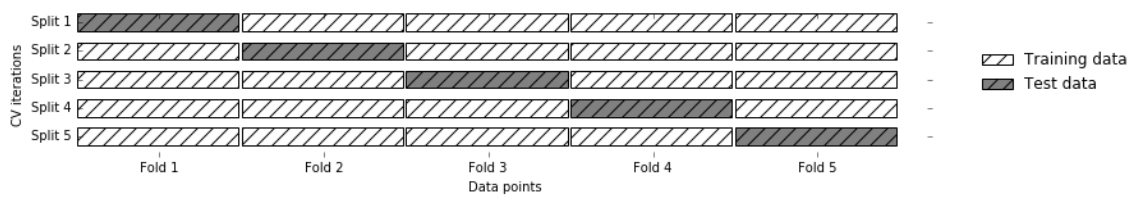
\includegraphics[scale=0.55]{Imagen_Machine/Validacion1}
	\caption{División de la data en validación cruzada con 5-fold}
	\label{Validacion1}
\end{figure}




Por lo general, el primer quinto de los datos es el primer fold, el segundo quinto de los datos es el segundo  fold, y así sucesivamente.


\subsection{Validación cruzada  en scikit-learn}
				% verdad fundamental = ground-truth
				
La validación cruzada se implementa en {\ttfamily  scikit-learn} usando la función {\ttfamily cross\_val\_score} del módulo {\ttfamily  model\_selection}. Los parámetros de la función  {\ttfamily cross\_val\_score}  son el modelo que queremos evaluar, la data de entrenamiento y las etiquetas {\ttfamily ground-truth}.     


Vamos a evaluar  el modelo  {\ttfamily  LogisticRegression} en el conjunto de la data Iris:

\begin{lstlisting}%[frame=single]

In[4]:

   from sklearn.model_selection import cross_val_score
   from sklearn.datasets import load_iris
   from sklearn.linear_model import LogisticRegression
   iris = load_iris()
   logreg = LogisticRegression()
   scores = cross_val_score(logreg, iris.data, iris.target)
   print("Cross-validation scores: {}".format(scores))

Out[4]:
 
    Cross-validation scores: [ 0.961 0.922 0.958]

\end{lstlisting}



Por defecto,  {\ttfamily cross\_val\_score}  realiza tres-fold para la validación cruzada,
 devolviendo tres valores de exactitud. Podemos cambiar el número de  folds 
 cambiando el  parámetro {\ttfamily cv}:


\begin{lstlisting}%[frame=single]

In[5]:

   scores = cross_val_score(logreg, iris.data, iris.target, cv=5)
   print("Cross-validation scores: {}".format(scores))

Out[5]:
    
    Cross-validation scores: [ 1. 0.967 0.933 0.9 1. ]

\end{lstlisting}


Una forma común de resumir la exactitud   de la validación cruzada es calcular la media:

\begin{lstlisting}%[frame=single]

In[6]:

   print("Average cross-validation score: {:.2f}".format(scores.mean()))

Out[6]:

    Average cross-validation score: 0.96

\end{lstlisting}

Usando la media de validación cruzada podemos concluir que en general se espera que el modelo sea alrededor del 96\%  exacto  en promedio. Mirando las cinco puntuaciones producidas por la validación cruzada de 5-folds, también podemos concluir que hay una varianza relativamente alta en la exactitud entre los  folds, que van de 100\%   hasta 90\%  de  exactitud. 

Esto podría implicar que el modelo es muy dependiente de los folds  particulares utilizados para el entrenamiento, pero también podría ser sólo una consecuencia del tamaño del conjunto de datos, que en este caso es muy pequeño.


\subsubsection{Beneficios de la validación cruzada}

Hay varios beneficios al usar la validación cruzada en lugar de una sóla división para la data (en dos conjuntos, el de entrenamiento y el de prueba). Primero, recuerde que {\ttfamily train\_test\_split} realiza 
{\bf{división aleatoria}} de la data.  Imagine que somos "{}afortunados"{} al dividir aleatoriamente los datos, y
todos los ejemplos que son difíciles de clasificar terminan en el conjunto de entrenamiento.
En ese caso, el conjunto  de  prueba  solo contendrá ejemplos "{}fáciles"{}, y 
la  exactitud en el conjunto de prueba será alta, un poco real. Por el contrario, si somos "{}desafortunados"{}, podríamos haber obtenido  aleatoriamente todos los ejemplos difíciles de clasificar en el conjunto de prueba y, en consecuencia, se obtendrá un puntaje de exactitud es bajo, nuevamente poco real. Sin embargo, cuando se utiliza la validación cruzada, cada dato estará en el conjunto de entrenamiento exactamente una vez:  cada dato está en uno de los  folds, y cada  fold es el conjunto de prueba una vez. 


Por lo tanto, el modelo necesita generalizar bien a todas las muestras en el conjunto de datos para que todas las puntuaciones de validación cruzada (y su media) sean altas.  Teniendo  múltiples divisiones de los datos también proporciona información sobre lo sensible que es el modelo a la selección del conjunto de datos de entrenamiento.  Para la data Iris, vimos exactitudes entre 90\% y 100\%.  Este es un rango bastante amplio y nos proporciona una idea sobre cómo podría funcionar el modelo en el peor de los casos y en los mejores escenarios cuando se aplica a nuevos datos.

Otro beneficio de la validación cruzada en comparación con el uso de una sóla división de los datos, es
que usamos nuestros datos de manera más efectiva. Cuando usamos  {\ttfamily train\_test\_split}, usualmente usamos 75\% de los datos para el entrenamiento  y 25\% de los datos para evaluación. Cuando se usan 5-folds en  validación cruzada, en cada iteración podemos usar cuatro quintos de los datos (80\%) para ajustar el
modelo.  Cuando usamos la validación cruzada con 10-folds, podemos usar nueve décimas de los datos
(90\%) para ajustar al modelo. Con más datos generalmente dará como resultado modelos más precisos.


La principal desventaja de la validación cruzada es el aumento del costo computacional. Como estamos 
ahora entrenando k modelos en lugar de un sólo modelo, la validación cruzada será aproximadamente k
veces más lento en comparación con una sóla división de los datos.\\
% Zorrillo


\begin{minipage}[t]{0.2\textwidth}
	\centering\raisebox{\dimexpr \topskip-\height}{%
		
\includegraphics[width=\textwidth]{Imagen_Machine/Zorrillo}}
\end{minipage}%\hfill
\begin{minipage}[t]{0.75\textwidth} 
	{\scriptsize		
		Es importante tener en cuenta que la validación cruzada no es una forma de
		construir un modelo que se pueda aplicar a nuevos datos. Validación cruzada
		"{}No"{} devuelve un modelo. 		
		Al aplicar {\ttfamily cross\_val\_score}, múltiples los modelos se construyen internamente, pero el propósito de la validación cruzada es sólo para evaluar qué tan bien se generalizará un algoritmo dado, cuando es entrenado en un conjunto de datos específico.}
\end{minipage}\\




\subsection{Validación cruzada K-Fold estratificada y otras estrategias}

Dividir el conjunto de datos en k-folds  comenzando con la k-ésima   primera parte de los datos, 
descrito como en la sección anterior, puede que no siempre sea una buena idea. Por ejemplo, vamos
echar un vistazo a la data Iris:

% {\ttfamily cross\_val\_score} 


\begin{lstlisting}%[frame=single]

In[7]:

   from sklearn.datasets import load_iris
   iris = load_iris()
   print("Iris labels:\n{}".format(iris.target))

Out[7]:

    Iris labels:
    [0 0 0 0 0 0 0 0 0 0 0 0 0 0 0 0 0 0 0 0 0 0 0 0 0 0 0 0 0 0 0 0 0 0 0 0 0
     0 0 0 0 0 0 0 0 0 0 0 0 0 1 1 1 1 1 1 1 1 1 1 1 1 1 1 1 1 1 1 1 1 1 1 1 1
     1 1 1 1 1 1 1 1 1 1 1 1 1 1 1 1 1 1 1 1 1 1 1 1 1 1 2 2 2 2 2 2 2 2 2 2 2
     2 2 2 2 2 2 2 2 2 2 2 2 2 2 2 2 2 2 2 2 2 2 2 2 2 2 2 2 2 2 2 2 2 2 2 2 2
     2 2]

\end{lstlisting}


Como puede ver, el primer tercio de los datos es la clase 0, el segundo tercio es la clase 1,
y el último tercio es la clase 2. Imagine hacer una validación cruzada con 3-fold  en esta data.
El primer fold sería sólo de clase 0, por lo que en la primera división de los datos, el conjunto de prueba sería sólo clase 0, y el conjunto de entrenamiento sería sólo clases 1 y 2.   Como las clases de entrenamiento y pruebas serían diferentes en las tres divisiones, las tres
medidas de exactitud  de la validación cruzada sería cero en este conjunto de datos. Eso no es muy útil, cómo  podemos obtener una mejor  de exactitud en la data Iris. 

Como la simple estrategia de k-fold falla aquí, {\ttfamily scikit-learn}  no la usa para clasificación, sino que utiliza estratificación de k -fold para la validación cruzada.
La validación cruzada estratificada,  dividen los datos de manera que las proporciones entre clases sean las mismas en cada fold, de acuerdo como están distribuidas en todo el conjunto de datos, en la  Figura \ref{Validacion2}  se ilustra la idea: 

\begin{lstlisting}%[frame=single]

In[8]

   mglearn.plots.plot_stratified_cross_validation()
   
\end{lstlisting}

\begin{figure}[h!]
	\centering
	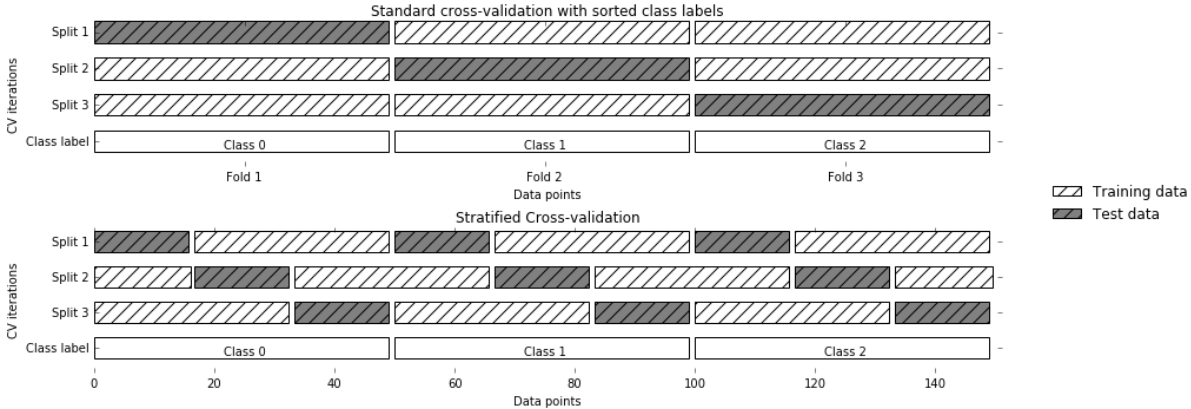
\includegraphics[scale=0.53]{Imagen_Machine/Validacion2}
	\caption{Comparación de validación cruzada estándar y validación cruzada estratificada
		cuando los datos se ordenan por etiqueta de clase}
	\label{Validacion2}
\end{figure}


Por ejemplo, si el 90\% de las  muestras pertenecen a la clase A y el 10\%  a 
pertenecen a la clase B, entoces  la validación cruzada estratificada asegura que en cada fold, haya el 90\% de las muestras pertenecen a la clase A y el 10\% de las muestras pertenecen a la clase B.

Por lo general, es una buena idea utilizar la validación cruzada de k-fold estratificada en lugar de k-fold
validación cruzada para evaluar un clasificador, porque produce resultados de estimaciones más confiables del rendimiento de generalización. 

En el caso de solo el 10\% de las muestras pertenecientes a la clase B, usando la validación cruzada estándar de k-fold, puede suceder fácilmente que sólo una contenga las  muestras de la clase A. 
El uso de este fold  como conjunto de prueba no sería muy informativo sobre el rendimiento general del clasificador.\\


Para la regresión, {\ttfamily scikit-learn} utiliza la validación cruzada k-fold estándar (standard k-fold cross-validation) de forma predeterminada. Eso sería posible también  tratar  de hacer que cada fold  sea representativo de los diferentes valores  que tiene el objetivo de regresión, pero esto no es una estrategia comúnmente utilizada y sería sorprendente para la mayoría de los usuarios.

\subsubsection{Más control sobre la validación cruzada}\label{VC}


Vimos anteriormente que podemos ajustar el número de folds que se usa  en {\ttfamily cross\_val\_score} mediante  el parámetro {\ttfamily cv}.   Sin embargo, {\ttfamily scikit-learn} permite un control mucho más fino sobre lo que sucede durante la división de la data al proporcionar un divisor de validación cruzada como el parámetro {\ttfamily cv}.  Para la mayoría de los casos de uso, los valores por defecto de la validación cruzada de k-fold para regresión y la  estratificado k-fold para clasificación funcionan bien, pero hay algunos casos en los que es posible que podria querer  utilizar una estrategia diferente; digamos, por ejemplo, que queremos usar la validación cruzada estándar k-fold en un conjunto 
de datos de clasificación para reproducir los resultados de otra persona.  Para esto, primero tenemos 
que importar la clase divisor de {\ttfamily KFold} desde el módulo {\ttfamily model\_selection} e instanciarla con el número de fold que  queremos usar:

\begin{lstlisting}%[frame=single]

In[9]:

   from sklearn.model_selection import KFold
   kfold = KFold(n_splits=5)

\end{lstlisting}


Entonces,  podemos pasar el objeto divisor {\ttfamily kfold} como el parámetro {\ttfamily cv} a {\ttfamily cross\_val\_score}:

\begin{lstlisting}%[frame=single]

In[10]:
  
   print("Cross-validation scores:\n{}".format(
          cross_val_score(logreg, iris.data, iris.target, cv=kfold)))

Out[10]:
    
    Cross-validation scores:
    [ 1. 0.933 0.433 0.967 0.433]

\end{lstlisting}

De esta forma, podemos verificar que es realmente una mala idea usar tres-fold (no estratificado) para la  validación cruzada en la data Iris:

\begin{lstlisting}%[frame=single]

In[11]:

   kfold = KFold(n_splits=3)
   print("Cross-validation scores:\n{}".format(
          cross_val_score(logreg, iris.data, iris.target, cv=kfold)))

Out[11]:

    Cross-validation scores:
    [ 0. 0. 0.]

\end{lstlisting}


Recuerde: cada  fold   corresponde a una de las clases del conjunto de data Iris, por lo que no se puede aprender nada. Otra forma de resolver este problema es barajando (aleatorio) los datos, en lugar de estratificar los folds, para eliminar o remover el orden de las muestras por etiqueta. Podemos hacerlo configurando el parámetro {\ttfamily shuffle} de {\ttfamily  KFold} como {\ttfamily True}. Si barajamos los datos, también necesitamos arreglar el estado aleatorio {\ttfamily random\_state} para obtener un barajamiento reproducible. De lo contrario, cada ejecución de {\ttfamily cross\_val\_score} daría un resultado diferente, ya que cada vez que  se use generá una división diferente (esto podría no ser un problema, pero puede  sorprender). Barajando los datos antes de dividirlos se obtiene un resultado mucho mejor:

\begin{lstlisting}%[frame=single]

In[12]:
   
   kfold = KFold(n_splits=3, shuffle=True, random_state=0)
   print("Cross-validation scores:\n{}".format(
          cross_val_score(logreg, iris.data, iris.target, cv=kfold)))
   
Out[12]:

    Cross-validation scores:
    [ 0.9 0.96 0.96]
    
\end{lstlisting}


\subsubsection{Validación cruzada de dejando uno fuera	\\ Leave-one-out} 


Otro método de validación cruzada frecuentemente usado es {\emph{dejar-uno-fuera (leave-one-out)}}, implementado en {\ttfamily LeaveOneOut}. Puedes pensar en la validación cruzada dejar-uno-fuera,  como una validación cruzada de k-fold donde cada fold  es una sóla muestra. Para cada división,  elige un sólo punto de la data para ser el conjunto de prueba. Esto puede llevar mucho tiempo, especialmente para grandes conjuntos de datos, pero a veces proporciona mejores estimaciomes en conjuntos pequeños:


\begin{lstlisting}%[frame=single]

In[13]:

   from sklearn.model_selection import LeaveOneOut
   loo = LeaveOneOut()
   scores = cross_val_score(logreg, iris.data, iris.target, cv=loo)
   print("Number of cv iterations: ", len(scores))
   print("Mean accuracy: {:.2f}".format(scores.mean()))

Out[13]:

    Number of cv iterations: 150
    Mean accuracy: 0.95

\end{lstlisting}



En la  validación cruzada dejando uno fuera o Leave-one-out cross-validation (Loovc) implica separar los datos de forma que para cada iteración tengamos una sola muestra para los datos de prueba y todo el resto conformando los datos de entrenamiento. La evaluación viene dada por el error, y en este tipo de validación cruzada el error es muy bajo, pero en cambio, a nivel computacional es muy costoso, puesto que se tienen que realizar un elevado número de iteraciones, tantas como N muestras tengamos y para cada una analizar los datos tanto de entrenamiento como de prueba.




\subsubsection{Validación cruzada Shuffle-split} 

%     Shuffle-split cross-validation



Otra estrategia muy flexible para la validación cruzada es la validación cruzada de  {\ttfamily shuffle-split}.  En la validación cruzada {\ttfamily shuffle-split}, cada muestra dividida tiene muchos puntos tanto para el conjunto de entrenamiento  {\ttfamily  train\_size} como para conjunto de prueba {\ttfamily test\_size} (disjuntos). Esta división es repetida {\ttfamily  n\_iter} veces. La Figura \ref{Barajar} ilustra una ejecución con cuatro iteraciones para dividir una data que consta de 10 puntos, en  el conjunto de entrenamiento con 5 puntos y el de pruebas con  2 puntos (puede usar enteros para {\ttfamily  train\_size}  y {\ttfamily test\_size} para usar tamaños absolutos para estos conjuntos, o números de punto flotante  (floating-point)  para usar fracciones de todo el conjunto de datos).


\begin{lstlisting}%[frame=single]

In[14]:

   mglearn.plots.plot_shuffle_split()

\end{lstlisting}


\begin{figure}[h!]
	\centering
	%
\includegraphics[scale=0.55]{../Imagen_Machine/Barajar}
	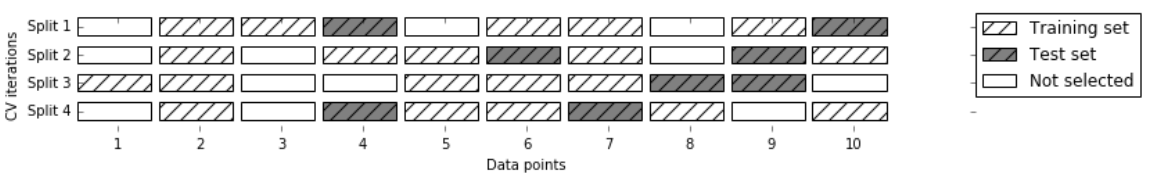
\includegraphics[scale=0.55]{Imagen_Machine/Barajar.png}
	\caption{ {\ttfamily ShuffleSplit} con 10 puntos, {\ttfamily train\_size=5,  test\_size=2},  y  {\ttfamily  n\_iter=4}}
	\label{Barajar}
\end{figure}



El siguiente código divide el conjunto de datos en un 50\% para la data de entrenamiento y 
 50\% para el de pruebas con 10 iteraciones:


\begin{lstlisting}%[frame=single]

In[15]:

   from sklearn.model_selection import ShuffleSplit
   shuffle_split = ShuffleSplit(test_size=.5, train_size=.5, n_splits=10)
   scores = cross_val_score(logreg, iris.data, iris.target, cv=shuffle_split)
   print("Cross-validation scores:\n{}".format(scores))
   
Out[15]:

   Cross-validation scores:
   [ 0.96 0.907 0.947 0.96 0.96 0.907 0.893 0.907 0.92 0.973]
  
\end{lstlisting}

La validación cruzada de Shuffle-split permite controlar el número de iteraciones independientemente de los tamaños de entrenamiento y prueba, lo que a veces puede ser útil. También permite usar sólo una parte de los datos en cada iteración, proporcionando configuraciones para {\ttfamily train\_size}  y  {\ttfamily test\_size} que no suman uno.  Submuestreando la data de esta manera, puede ser útil para experimentar con grandes conjuntos de datos.\\

 También hay una variante estratificada de {\ttfamily  ShuffleSplit}, acertadamente llamada {\ttfamily  StratifiedShuffleSplit}, que puede proporcionar resultados más fiables para las tareas de clasificación.



\subsubsection{Validación cruzada con grupos}



Otra configuración muy común para la validación cruzada es cuando hay grupos en la
data que están altamente relacionados. Digamos que quieres construir un sistema para reconocer emociones
a partir de imágenes de caras, y usted recopila un conjunto de datos de imágenes de 100 personas, donde cada
la persona es capturada varias veces, mostrando varias emociones. El objetivo es construir un
clasificador que pueda identificar correctamente las emociones de las personas que no están en el conjunto de datos.  Podrías usar la validación cruzada estratificada por defecto para medir el rendimiento de un clasificador. Sin embargo, es probable que las imágenes de la misma persona estén en ambos conjuntos, en el de entrenamiento y en el de prueba. Será mucho más fácil para un clasificador detectar emociones en una cara que es parte del conjunto de entrenamiento, en comparación con una cara completamente nueva.   Por lo tanto,  para evaluar la exactitud de generalización a nuevas caras,  debemos asegurarnos  que  los conjuntos de  entrenamiento y de prueba contienen imágenes de diferentes personas.\\

 
Para lograr esto, podemos usar {\ttfamily GroupKFold}, que toma un arreglo de grupos como argumento, que podemos usar para indicar qué persona está en la imagen. Los arrreglos de grupos aquí indican  grupos en la data  que no deben dividirse al crear los conjuntos de entrenamiento y prueba, y no debe confundirse con la etiqueta de clase. \\



 Este ejemplo de grupos en los datos es común en aplicaciones médicas, donde
pueden tener múltiples muestras del mismo paciente, pero están interesadas en generalizar
a nuevos pacientes. Del mismo modo, en el reconocimiento de voz, puede tener múltiples grabaciones
de la  misma persona en la data, pero el interés está centrado  en reconocer la voz de nuevas personas.\\


El siguiente es un ejemplo del uso de un conjunto de datos sintético con una agrupación dada por
un arreglo de grupos. La data  consta de 12 puntos,  para cada uno de los puntos, 
el grupos especifica a qué grupo (piensa en pacientes) pertenece el punto. Los grupos especifican
que hay cuatro grupos, y las primeras tres muestras pertenecen al primer grupo, las siguientes cuatro muestras pertenecen al segundo grupo, y así sucesivamente:

\begin{lstlisting}%[frame=single]

In[17]:

   from sklearn.model_selection import GroupKFold
   # create synthetic dataset
   X, y = make_blobs(n_samples=12, random_state=0)
   # assume the first three samples belong to the same group,
   # then the next four, etc.
   groups = [0, 0, 0, 1, 1, 1, 1, 2, 2, 3, 3, 3]
   scores = cross_val_score(logreg, X, y, groups, cv=GroupKFold(n_splits=3))
   print("Cross-validation scores:\n{}".format(scores))

Out[17]:

    Cross-validation scores:
    [ 0.75 0.8 0.667]

\end{lstlisting}


Las muestras no necesitan ser ordenadas por grupo; simplemente hicimos esto con propósito de ilustrar. Las divisiones son calculadas en base a estas etiquetas que se visualizan en la Figura \ref{GrupoArray}.

\begin{lstlisting}%[frame=single]

In[17]:

mglearn.plots.plot_label_kfold()


\end{lstlisting}%[frame=single]


\begin{figure}[h!]
	\centering
	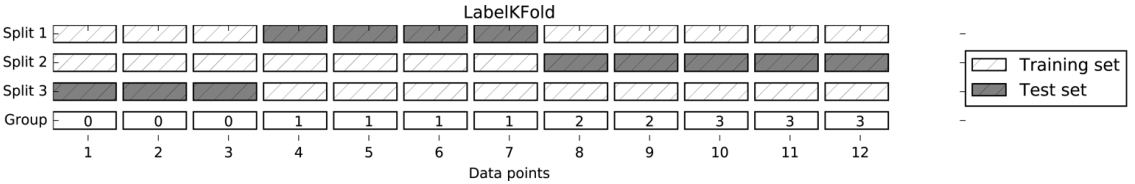
\includegraphics[scale=0.55]{Imagen_Machine/GrupoArray}
	\caption{División dependiente de etiquetas con {\ttfamily GroupKFold}}
	\label{GrupoArray}
\end{figure}

%    Label-dependent splitting with GroupKFold


Como puede ver, por cada división (split $i$), cada grupo está completamente en el conjunto de entrenamiento o completamente en el conjunto de pruebas.


Hay más estrategias de división para la validación cruzada en {\ttfamily scikit-learn}, que permiten una mayor variedad de casos de uso (puede encontrar estos en la guía del usuario de \href{https://scikit-learn.org/stable/modules/cross_validation.html}{\textcolor{red}{\ttfamily scikit-learn}}). Sin embargo, el estándar  {\ttfamily KFold, StratifiedKFold} y  {\ttfamily  GroupKFold } son los más comunmente usados.


\subsubsection{Búsqueda de cuadrícula}

%    Grid Search

Ahora que sabemos cómo evaluar qué tan bien generaliza un modelo, podemos tomar el
siguiente paso y mejorar el rendimiento de generalización del modelo ajustando sus parámetros.  Discutimos la configuración de parámetros de muchos de los algoritmos en 
en los capítulos \ref{Cap2}  y  \ref{Cap3}, y su importancia de entender qué significan los parámetros
antes de intentar ajustarlos. 

 
Encontrar los valores de los parámetros importantes de un  modelo (los que proporcionan el mejor rendimiento de generalización) es una tarea difícil, pero necesario para casi todos los modelos y conjuntos de datos. Debido a que es una tarea tan común,   {\ttfamily scikit-learn} proporciona  métodos estándar  para ayudarte con esto.  El método    más común es la búsqueda de cuadrícula (grid search), que básicamente significa probar todas las combinaciones posibles de parámetros de interés. 


Considere el caso de un kernel SVM con un kernel RBF (función de base radial), como
es implementado en la clase SVC. Como discutimos en el Capítulo \ref{Cap2}, hay dos 
parámetros  importantes: el ancho de banda del kernel, gamma, y el parámetro C  de regularización.  Digamos que desea probar los valores 0.001, 0.01, 0.1, 1, 10 y 100 para el parámetro C, y los mismos valores para gamma.

Ya que tenemos seis configuraciones diferentes para C y gamma  que queremos probar,  tenemos 36 combinaciones de parámetros en total. Observando todas las combinaciones posibles se crea una tabla (o cuadrícula) de configuraciones de parámetros para el SVM, como se muestra aquí:

\hspace{-0.6cm}  
\vspace{-0.6cm} 
\begin{figure}[h!]
	%\centering
	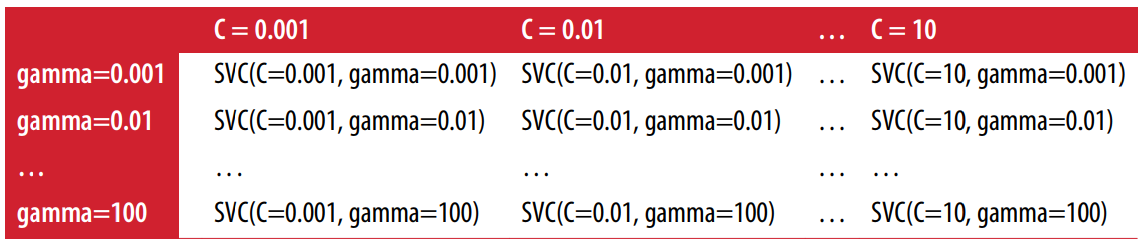
\includegraphics[scale=0.55]{Imagen_Machine/TablaGrid}
\end{figure}\label{TablaGrid} 

%  \ref{TablaGrid}


\subsubsection{Búsqueda de cuadrícula simple}\label{Gsear}

 Podemos implementar una búsqueda de cuadrícula simple al igual que para bucles sobre los dos parámetros, entrenando y evaluando un clasificador para cada combinación:  

\begin{lstlisting}%[frame=single]

In[18]:
   
   # naive grid search implementation
   from sklearn.svm import SVC
   X_train, X_test, y_train, y_test = train_test_split(
       iris.data, iris.target, random_state=0)
   print("Size of training set: {} size of test set: {}".format(
          X_train.shape[0], X_test.shape[0]))
          
   best_score = 0
   
   for gamma in [0.001, 0.01, 0.1, 1, 10, 100]:
       for C in [0.001, 0.01, 0.1, 1, 10, 100]:
           # for each combination of parameters, train an SVC
           svm = SVC(gamma=gamma, C=C)
           svm.fit(X_train, y_train)
           # evaluate the SVC on the test set
           score = svm.score(X_test, y_test)
           # if we got a better score, store the score and parameters
           if score > best_score:
              best_score = score
              best_parameters = {'C': C, 'gamma': gamma}
              
   print("Best score: {:.2f}".format(best_score))
   print("Best parameters: {}".format(best_parameters))

Out[18]:
   
    Size of training set: 112 size of test set: 38
    Best score: 0.97
    Best parameters: {'C': 100, 'gamma': 0.001}

\end{lstlisting}


\subsubsection{El peligro de sobreajustar los parámetros y el conjunto de validación}


Dado este resultado, podríamos intentar de reportar que encontramos un modelo que funciona
con un 97\% de exactitud en la data.  Sin embargo, esta afirmación podría ser demasiado optimista (o simplemente mal), por la siguiente razón: probamos  muchos parámetros diferentes y seleccionó el que tiene la mejor exactitud en el conjunto de prueba, pero esta exactitud no necesariamente es transferida a nuevos datos. Debido a que utilizamos los datos de prueba para ajustar los parámetros,  ya no podemos usarlo para evaluar lo bueno que es el modelo.  

Esta es la misma razón por la que necesitábamos dividir los datos en conjuntos de entrenamiento y prueba en primer lugar; ahora  necesitamos un conjunto independiente de datos para evaluar, uno que no se haya usado para construir el modelo.


Una forma de resolver este problema es dividir los datos nuevamente, por lo que tenemos tres conjuntos:
un conjunto de entrenamiento para construir el modelo, uno de validación (o desarrollo) para seleccionar el parámetros del modelo y el de prueba para evaluar el rendimiento de los parámetros seleccionados.  En la figura \ref{Triple}  muestra cómo se ve esto:


\begin{lstlisting}%[frame=single]

In[19]:

mglearn.plots.plot_threefold_split()


\end{lstlisting}


\begin{figure}[h!]
	\centering
	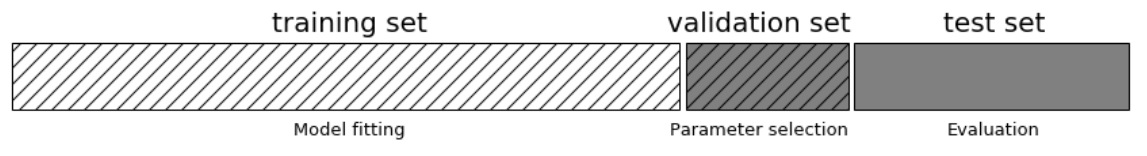
\includegraphics[scale=0.55]{Imagen_Machine/Triple}
	\caption{Una división triple-fold  de la data, en un conjunto de entrenamiento, uno de validación y el otro para prueba}
	\label{Triple}
\end{figure}


Después de seleccionar los mejores parámetros usando el conjunto de validación, podemos reconstruir un modelo usando los parámetros que encontramos, pero ahora entrenando tanto en los datos de entrenamiento como en los datos de validación. De esta manera, podemos utilizar la mayor cantidad de datos posible para construir el modelo. Esto conduce a la siguiente implementación: 

\begin{lstlisting}%[frame=single]

In[20]:

   from sklearn.svm import SVC
   # split data into train+validation set and test set
   X_trainval, X_test, y_trainval, y_test = train_test_split(
       iris.data, iris.target, random_state=0)
   # split train+validation set into training and validation sets
   X_train, X_valid, y_train, y_valid = train_test_split(
       X_trainval, y_trainval, random_state=1)
   print("Size training set: {} size validation set: {} size test set:" 
         " {}\n".format(X_train.shape[0], X_valid.shape[0], X_test.shape[0]))
         
   best_score = 0

   for gamma in [0.001, 0.01, 0.1, 1, 10, 100]:
       for C in [0.001, 0.01, 0.1, 1, 10, 100]:
       # for each combination of parameters, train an SVC
       svm = SVC(gamma=gamma, C=C)
       svm.fit(X_train, y_train)
       # evaluate the SVC on the test set
       score = svm.score(X_valid, y_valid)
       # if we got a better score, store the score and parameters
       if score > best_score:
          best_score = score
          best_parameters = {'C': C, 'gamma': gamma}
          
   # rebuild a model on the combined training and validation set,
   # and evaluate it on the test set
   svm = SVC(**best_parameters)
   svm.fit(X_trainval, y_trainval)
   test_score = svm.score(X_test, y_test)
   print("Best score on validation set: {:.2f}".format(best_score))
   print("Best parameters: ", best_parameters)
   print("Test set score with best parameters: {:.2f}".format(test_score))

Out[20]:
   
   Size of training set: 84 size of validation set: 28 size of test set: 38
   Best score on validation set: 0.96
   Best parameters: {'C': 10, 'gamma': 0.001}
   Test set score with best parameters: 0.92

\end{lstlisting}

El mejor puntaje (score) en el conjunto de validación es 96\%: ligeramente más bajo que antes, probablemente
porque usamos menos datos para entrenar el modelo ({\ttfamily X\_train} es más pequeño ahora porque dividimos la data dos veces). Sin embargo, la puntuación en el conjunto de pruebas, que realmente nos dice qué tan bien generalizamos, es aún más bajo, al 92\%. Así, que sólo podemos afirmar que la  clasificación con  nuevos datos correctamente  se de  92\% , y no del 97\%  como pensábamos antes!

La distinción entre el conjunto de entrenamiento, el de validación y el de prueba es fundamentalmente importante para aplicar métodos de aprendizaje automático en la práctica. Cualquier elección realizada en la  exactitud del conjunto de prueba  "{}fuga"{}  información del conjunto de prueba al modelo.   Por lo tanto, es importante mantener un conjunto de pruebas separado, que sólo se utilice  para la evaluación final.

 Es una buena práctica hacer todos los análisis exploratorios y la selección de modelos utilizando
la combinación de un conjunto de entrenamiento y validación, y reservar el conjunto de prueba para la evaluación  final, esto es incluso cierto para la visualización exploratoria.  Estrictamente hablando, evaluando más de un modelo en el conjunto de prueba y  eligiendo el mejor, resultaría  una estimación demasiado optimista de la exactitud del modelo.


\subsubsection{Búsqueda de cuadrícula con validación cruzada}

El método de dividir la data en los conjuntos de entrenamiento, validación y   prueba
que acabamos de ver es factible, y de uso relativamente común, pero es muy sensible  a cómo se dividen exactamente los datos. 

De la salida del fragmento de código anterior podemos ver que {\ttfamily GridSearchCV} selecciona {\ttfamily  'C': 10, y   'gamma':  0.001},   como los mejores parámetros;  mientras que la salida del código en la sección anterior selecciona a {\ttfamily 'C': 100,   y   'gamma': 0.001},  como los mejores parámetros.  

Para una mejor estimación del rendimiento de la generalización, en lugar de utilizar una única división en un conjunto de entrenamiento y  validación, podemos utilizar la validación cruzada para evaluar el rendimiento de cada combinación de parámetros. Este método puede codificarse como sigue:


\begin{lstlisting}%[frame=single]

In[21]:

   for gamma in [0.001, 0.01, 0.1, 1, 10, 100]:
       for C in [0.001, 0.01, 0.1, 1, 10, 100]:
       # for each combination of parameters,
       # train an SVC
       svm = SVC(gamma=gamma, C=C)
       # perform cross-validation
       scores = cross_val_score(svm, X_trainval, y_trainval, cv=5)
       # compute mean cross-validation accuracy
       score = np.mean(scores)
       # if we got a better score, store the score and parameters
       if score > best_score:
          best_score = score
          best_parameters = {'C': C, 'gamma': gamma}          
   # rebuild a model on the combined training and validation set
   svm = SVC(**best_parameters)
   svm.fit(X_trainval, y_trainval)

\end{lstlisting}


Para evaluar la exactitud del SVM con un ajuste particular de  C  y  gamma  mediante  la validación cruzada de 5-fold, necesitamos entrenar  36 * 5  =  180  modelos.  Como se puede imaginar, el principal inconveniente del uso de la validación cruzada es el tiempo que se tarda en entrenar todos estos modelos. 

La siguiente visualización (Figura \ref{Grid1}) ilustra cómo se selecciona el mejor parámetro en el código anterior: 


\begin{lstlisting}%[frame=single]

In[22]:

   mglearn.plots.plot_cross_val_selection()

\end{lstlisting}


	\begin{figure}[h!]
	\centering
	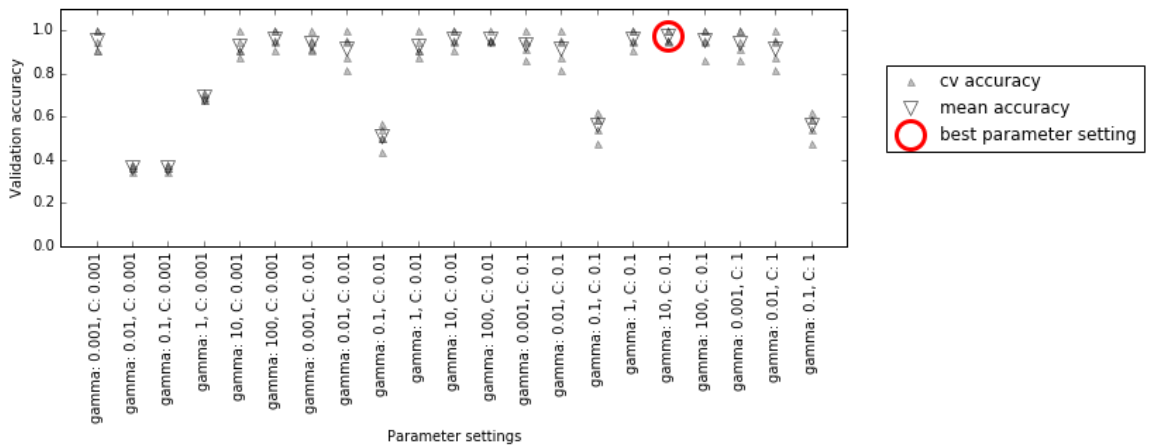
\includegraphics[scale=0.55]{Imagen_Machine/Grid1}
	\caption{Resultados de  búsqueda en cuadrícula con validación cruzada}
	\label{Grid1}
    \end{figure}


Para cada cofiguración de parámetros (sólo se muestra un subconjunto), se calculan cinco valores de exactitud, uno para cada división en la validación cruzada. Luego se calcula la exactitud media de validación para cada parámetro configuardo. Se eligen los parámetros con la mayor exactitud media de validación, marcados por el círculo.\\


\begin{minipage}[t]{0.2\textwidth}
	\centering\raisebox{\dimexpr \topskip-\height}{%
		
\includegraphics[width=\textwidth]{Imagen_Machine/Escorpion}}
\end{minipage}%\hfill
\begin{minipage}[t]{0.75\textwidth} 
	{\scriptsize		
Como hemos dicho antes, la validación cruzada es una manera de evaluar  cierto algoritmo en una 
data específica. Sin embargo, esto es  frecuentemente usado en conjunsión con métodos de búsqueda de 
parámetros como   búsqueda en cuadrícula (grid search). Por esta razón, muchas personas utilizan el término 
validación cruzada coloquialmente para referirse a la búsqueda de cuadrícula con  validación cruzada.}
\end{minipage} 
\vspace{0.5cm}

El proceso general de dividir los datos, corriendo el método grid search (la búsqueda de cuadrícula) y la  evaluación final  de los parámetros se ilustran en la Figura \ref{GridSearchCV2}:

\begin{lstlisting}%[frame=single]

In[23]:

   mglearn.plots.plot_grid_search_overview()
   
\end{lstlisting}


\begin{figure}[h!]
	\centering
	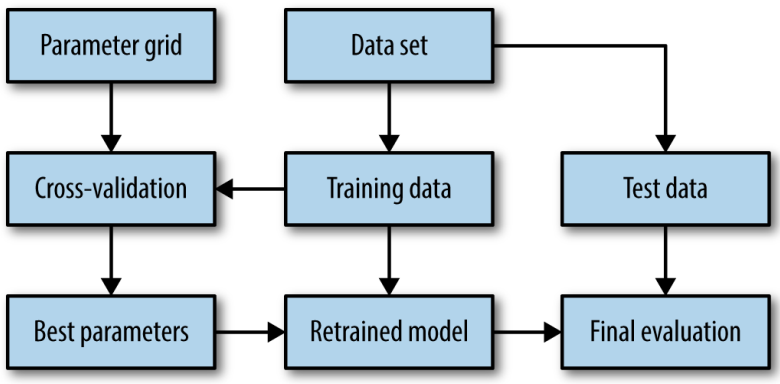
\includegraphics[scale=0.55]{Imagen_Machine/GridSearchCV2}
	\caption{Descripción general del proceso de selección de parámetros y evaluación del modelo con
		GridSearchCV}
	\label{GridSearchCV2}
\end{figure}


Debido a que  grid search   (búsqueda de cuadrícula) con validación cruzada es un método  comúnmente muy utilizado para ajustar parámetros,  {\ttfamily scikit-learn} proporciona la clase {\ttfamily GridSearchCV}, que la implementa en  forma de un estimador.
Para usar la clase {\ttfamily GridSearchCV}, primero debe especificar los parámetros que 
desea buscar utilizando un diccionario.   {\ttfamily GridSearchCV}  realizará todos los ajustes de modelo necesarios. Las claves del diccionario son los nombres de los parámetros que queremos ajustar (como se indica al construir el modelo, en este caso, C y gamma), y los valores son los parámetros que queremos probar.

Probando los valores  0.001, 0.01, 0.1, 1, 10 y 100 para  C  y  gamma se traducen en el siguiente
diccionario:


\begin{lstlisting}%[frame=single]

In[24]:

   param_grid = {'C': [0.001, 0.01, 0.1, 1, 10, 100],
                 'gamma': [0.001, 0.01, 0.1, 1, 10, 100]}
   print("Parameter grid:\n{}".format(param_grid))

Out[24]:

    Parameter grid:
    {'C': [0.001, 0.01, 0.1, 1, 10, 100], 'gamma': [0.001, 0.01, 0.1, 1, 10, 100]}

\end{lstlisting}


Ahora podemos instanciar la clase {\ttfamily  GridSearchCV} con el modelo (SVC), para buscar el parámetro
grid  ({\ttfamily  param\_grid}) y la estrategia de validación cruzada que queremos usar (por ejemplo, validación cruzada estratificada de cinco-fold):


\begin{lstlisting}%[frame=single]

In[25]:
   
   from sklearn.model_selection import GridSearchCV
   from sklearn.svm import SVC
   grid_search = GridSearchCV(SVC(), param_grid, cv=5)

\end{lstlisting}

{\ttfamily  GridSearchCV} utilizará la validación cruzada en lugar de la división en los conjuntos de entrenamiento y validación que usamos antes. Sin embargo, aún necesitamos dividir los datos en
 dos conjuntos, el de entrenamiento y   prueba, para evitar sobreajustar los parámetros:

\begin{lstlisting}%[frame=single]

In[26]:

   X_train, X_test, y_train, y_test = train_test_split(
       iris.data, iris.target, random_state=0)

\end{lstlisting}

El objeto {\ttfamily  grid\_search} que creamos se comporta como un clasificador; podemos llamar al
 métodos estándar {\ttfamily fit,  predict} y {\ttfamily  score} en él{\footnote{\scriptsize  Un estimador en {\ttfamily scikit-learn}  creado  a partir de otro estimador es llamado  meta-estimator. El {\ttfamily GridSearchCV} es el  comúnmente más  usado, pero lo veremos más adelante.}}.  
 Sin embargo, cuando llamamos {\ttfamily fit},  este corre la validación cruzada para cada combinación de parámetros que especificamos en {\ttfamily param\_grid}:

\begin{lstlisting}%[frame=single]

In[27]:

   grid_search.fit(X_train, y_train)

\end{lstlisting}

Ajustando  el objeto  {\ttfamily GridSearchCV} no sólo busca los mejores parámetros, sino que también
ajusta automáticamente un nuevo modelo en todo el conjunto de entrenamiento con los parámetros que
produjo el mejor rendimiento de validación cruzada. 

Por lo tanto, lo que sucede en {\ttfamily fit} es equivalente al resultado del código In[21] que vimos al comienzo de esta sección. La clase {\ttfamily GridSearchCV}  proporciona una interfaz muy conveniente para acceder al reentrenamiento modelo usando los métodos {\ttfamily predict}  y  {\ttfamily score}. 

Para evaluar qué tan bien  generalizar  el mejor parámetro encontrado, podemos correr {\ttfamily score} 
sobre el conjunto de prueba:

\begin{lstlisting}%[frame=single]

In[28]:

   print("Test set score: {:.2f}".format(grid_search.score(X_test, y_test)))

Out[28]:
    
    Test set score: 0.97

\end{lstlisting}

 
Seleccionando los  parámetros mediante validación cruzada, en realidad encontramos un modelo que logró
 97\% de exactitud sobre  el conjunto de prueba. Lo importante aquí, es que no se usó  el
conjunto de prueba para elegir los parámetros.

Los parámetros encontrados se anotan en el atributo {\ttfamily  best\_params\_} y la mejor exactitud de validación cruzada (la exactitud media sobre las diferentes divisiones para esta configuración de parámetros)  se almacena en {\ttfamily best\_score\_}:


\begin{lstlisting}%[frame=single]

In[29]:

   print("Best parameters: {}".format(grid_search.best_params_))
   print("Best cross-validation score: {:.2f}".format(grid_search.best_score_))

Out[29]:

    Best parameters: {'C': 100, 'gamma': 0.01}
    Best cross-validation score: 0.97

\end{lstlisting}


\begin{minipage}[t]{0.2\textwidth}
	\centering\raisebox{\dimexpr \topskip-\height}{%
		
\includegraphics[width=\textwidth]{Imagen_Machine/Zorrillo}}
\end{minipage}%\hfill
\begin{minipage}[t]{0.75\textwidth} 
	{\scriptsize		
	Nuevamente, hay que tener cuidado de no confundir {\ttfamily best\_score\_} con la generalización.
	rendimiento del modelo calculado por el método de {\ttfamily score } en el conjunto
	 de prueba. Usando el método de {\ttfamily score } (o evaluar la salida del método {\ttfamily predict})  se emplea un modelo entrenado en todo el conjunto de entrenamiento.   El atributo  {\ttfamily best\_score\_}  almacena exactitud media de la validación cruzada,  con la validación cruzada realizada en el conjunto de entrenamiento.}
\end{minipage}\\

A veces es útil tener acceso al modelo real que se encontró, por ejemplo, para ver los coeficientes o características importantes. Puede acceder al modelo con los mejores parámetros entrenados en todo el conjunto de entrenamiento utilizando el atributo {\ttfamily best\_estimator\_}:


\begin{lstlisting}%[frame=single]

In[30]:

   print("Best estimator:\n{}".format(grid_search.best_estimator_))

Out[30]:

    Best estimator:
    SVC(C=100, cache_size=200, class_weight=None, coef0=0.0,
       decision_function_shape=None, degree=3, gamma=0.01, kernel='rbf',
       max_iter=-1, probability=False, random_state=None, shrinking=True,
       tol=0.001, verbose=False)

\end{lstlisting}

Debido a que {\ttfamily grid\_search} tiene métodos de predicción y puntuación, el uso de {\ttfamily best\_estimator\_} no es necesario para hacer predicciones o evaluar el modelo.


\subsubsection{Analizando el resultado de la validación cruzada}


A menudo es útil visualizar los resultados de la validación cruzada,  para entender  cómo la  generalización del modelo depende de los parámetros que estamos buscando. Como las búsquedas de cuadrícula son muy costosos desde desde el punto de vista computacional, es una buena idea comenzar con una relación de cuadrícula relativamente robusta y pequeña.   %  gruesa   coarse  grueso
Luego podemos inspeccionar los resultados de la validación cruzada con grid search
(búsqueda de cuadrícula), y posiblemente ampliar esta búsqueda. Los resultados de una búsqueda  cuadrícula  pueden ser encontrados en el atributo {\ttfamily cv\_results\_}, que es un diccionario que almacena todos los aspectos de la búsqueda. 

Este contiene muchos detalles, como se pueden ver en el siguiente resultado, y se ve mejor
después de convertirlo en una DataFrame de {\ttfamily pandas}:


\begin{lstlisting}

In[31]:

   import pandas as pd
   # convert to DataFrame
   results = pd.DataFrame(grid_search.cv_results_)
   # show the first 5 rows
   display(results.head())

Out[31]:

       param_C  param_gamma  params                        mean_test_score
   0   0.001    0.001        {'C': 0.001, 'gamma': 0.001}       0.366
   1   0.001     0.01        {'C': 0.001, 'gamma': 0.01}        0.366
   2   0.001      0.1        {'C': 0.001, 'gamma': 0.1}         0.366
   3   0.001        1        {'C': 0.001, 'gamma': 1}           0.366
   4   0.001       10        {'C': 0.001, 'gamma': 10}          0.366

     rank_test_score split0_test_score split1_test_score split2_test_score
           
   0      22                0.375            0.347            0.363
   1      22                0.375            0.347            0.363
   2      22                0.375            0.347            0.363
   3      22                0.375            0.347            0.363
   4      22                0.375            0.347            0.363
           
          split3_test_score   split4_test_score   std_test_score
           
   0           0.363               0.380             0.011
   1           0.363               0.380             0.011
   2           0.363               0.380             0.011
   3           0.363               0.380             0.011
   4           0.363               0.380             0.011
    
\end{lstlisting}



Cada fila en el resultado corresponde a una configuración  particular del parámetro. Para 
cada conjunto, se registran los resultados de todas las divisiones de validación cruzada, así 
como la media y desviación estándar sobre todas las divisiones. 

La tabla o cuadrícula bidimensional de parámetros (C y gamma),  se visualiza mejor como un mapa
caliente, como se muestra en la figura \ref{MapaCG}.  Primero  extraemos los scores o puntajes
 promedio  de validación, luego  remodelamos o rediseñamos los puntajes o scores  para que los 
 ejes  corresponda con   C  y   gamma:

\begin{lstlisting}%[frame=single]


In[32]:

   scores = np.array(results.mean_test_score).reshape(6, 6)

   # plot the mean cross-validation scores
   mglearn.tools.heatmap(scores, xlabel='gamma', 
                         xticklabels=param_grid['gamma'],
                         ylabel='C', yticklabels=param_grid['C'],
                         cmap="viridis")

\end{lstlisting}



\begin{figure}[h!]
	\centering
	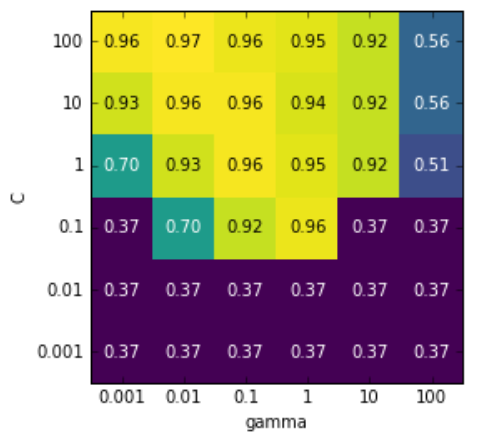
\includegraphics[scale=0.55]{Imagen_Machine/MapaCG}
	\caption{Mapa caliente  de la puntuación media de validación cruzada en función de C y gamma}
	\label{MapaCG}
\end{figure}


Cada punto en el mapa caliente corresponde a una corrida de validación cruzada, con una configuaración particular de parámetros. El color codifica la exactitud de validación cruzada, con colores claros 
 significan alta exactitud y colores oscuros que significan baja exactitud.  Se puedes ver que  SVC es muy sensible a la configuración de los parámetros.  Para muchos de los parámetros configurados, la exactitud es de alrededor del 40\%, lo cual es bastante mala; para otras configuraciones, la exactitud es alrededor del 96\%.    Podemos obtener  de este grafico  varias conclusiones. Primero, los parámetros configurados   son muy importantes para obtener un buen rendimiento. Ambos parámetros (C y gamma) son muy importantes, ya que  ajustarlos puede cambiar la exactitud del 40\% a 96\%.   Además, los rangos que seleccionamos para los parámetros son rangos en los que se ven  cambios significativos en el resultado.  También es importante tener en cuenta que los rangos para los  parámetros son lo suficientemente grandes: los valores óptimos para cada parámetro no están  en los bordes del gráfico.\\

Ahora veamos algunos gráficos (ver Figura \ref{MapaCG2}) donde el resultado es menos ideal,
porque los rangos de búsqueda no se eligieron adecuadamente:


\begin{figure}[h!]
	\centering
	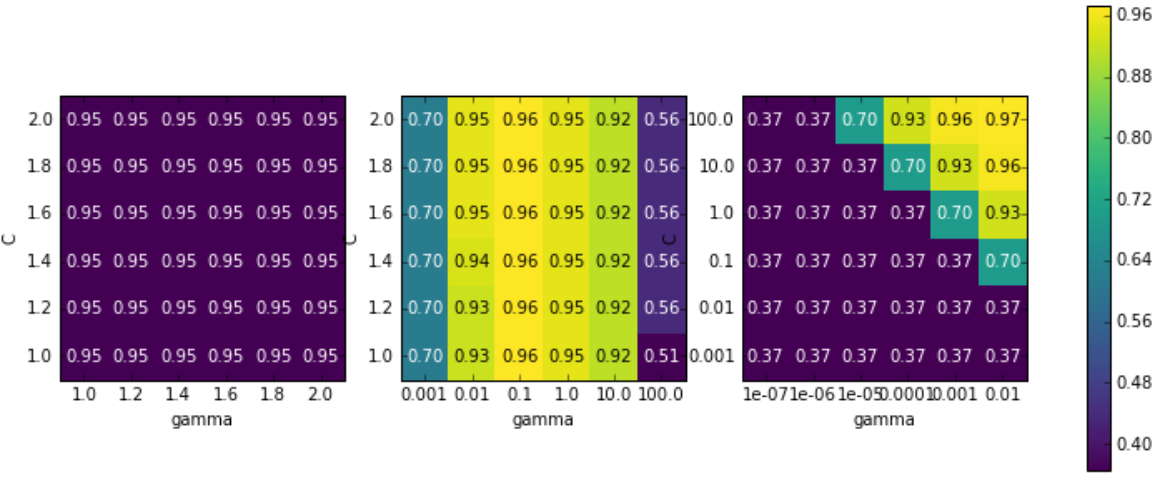
\includegraphics[scale=0.55]{Imagen_Machine/MapaCG2}
	\caption{Visualizaciones de mapas caliente de search grids mal especificadas}
	\label{MapaCG2}
\end{figure}




\begin{lstlisting}%[frame=single]

In[33]:

   fig, axes = plt.subplots(1, 3, figsize=(13, 5))
   
   param_grid_linear = {'C': np.linspace(1, 2, 6),
                        'gamma': np.linspace(1, 2, 6)}
                        
   param_grid_one_log = {'C': np.linspace(1, 2, 6),
                         'gamma': np.logspace(-3, 2, 6)}
                         
   param_grid_range = {'C': np.logspace(-3, 2, 6),
                       'gamma': np.logspace(-7, -2, 6)}
                       
   for param_grid, ax in zip([param_grid_linear, param_grid_one_log,
                              param_grid_range], axes):
       grid_search = GridSearchCV(SVC(), param_grid, cv=5)
       grid_search.fit(X_train, y_train)
       scores = grid_search.cv_results_['mean_test_score'].reshape(6, 6)
       
       # plot the mean cross-validation scores
       scores_image = mglearn.tools.heatmap(
           scores, xlabel='gamma', ylabel='C', xticklabels=param_grid['gamma'],
           yticklabels=param_grid['C'], cmap="viridis", ax=ax)
           
   plt.colorbar(scores_image, ax=axes.tolist())

\end{lstlisting}

El primer gráfico no muestra ningún cambio, con un color constante en toda la cuadrícula de parámetro.
En este caso, esto es causado por  la escala y rango incorrectos de los parámetros C y gamma.
Sin embargo, si no se observa ningún cambio en la exactitud sobre el parámetro con las diferentes
configuraciones, también podría ser que un parámetro simplemente no sea importante en lo
absoluto. Por lo general es bueno probar primero valores muy extremos, para ver si 
hay algún cambio en la exactitud como  resultado de cambiar un parámetro.\\

El segundo gráfico  muestra un patrón de rayas verticales. Esto indica que solo la configuración
del parámetro gamma hace alguna diferencia. Esto podría significar que el parámetro gamma
está buscando valores interesantes pero el parámetro C no lo está haciendo, o podría significar
que el parámetro C no es importante.\\

%   de esta frontera
El tercer gráfico muestra cambios en C y gamma. Sin embargo, podemos ver que en 
toda la parte inferior izquierda del gráfico, no pasa nada interesante. Probablemente podamos
excluir los valores muy pequeños en  futuras (grid searches)  búsquedas en la cuadrícula. 
La configuración  óptimo de parámetros  está en la parte superior derecha. Como el óptimo está en el borde de la gráfico, podemos esperar que haya algún o algunos valores mejores  más allá del borde, y podríamos querer cambiar nuestro rango de búsqueda para incluir más parámetros en esta región.\\


Ajustar los  parámetros de grid  basados   en función de las  puntuaciones (scores)  de validación cruzada está  perfectamente bien, y una buena manera de explorar la importancia de diferentes parámetros. Sin embargo, no debe probar diferentes rangos de parámetros en el conjunto de prueba final, como hemos discutido anteriormente, la evaluación del conjunto de prueba debe ocurrir sólo una vez que sabemos exactamente qué modelo queremos utilizar.


\subsubsection{Busqueda en espacios que no son cuadrículas}\label{Pagina1}




%   Search over spaces that are not grids

En algunos casos, intentar todas las combinaciones posibles de todos los parámetros como lo hace {\ttfamily  GridSearchCV}, no es una buena idea. Por ejemplo, SVC tiene un parámetro  kernel y
dependiendo de qué kernel  (o  núcleo) se elija, otros parámetros serán relevantes.    Si kernel = "{}linear"{}, el modelo es lineal y sólo se usa el parámetro C.  Si kernel = "{}rbf"{},
se utilizan los parámetros C y {\ttfamily  Gamma} (pero no otros parámetros como el grado). 
En este caso, la búsqueda en todas las combinaciones posibles de C, {\ttfamily  Gamma} y kernel no
tiene sentido:  si kernel = "{}linear"{}, no se usa {\ttfamily  Gamma} e intentar con  diferentes valores para
{\ttfamily  Gamma} sería una pérdida de tiempo. Para tratar con este tipo de parámetros "{}condicionales"{},
\: {\ttfamily GridSearchCV} permite que {\ttfamily param\_grid} sea una lista de diccionarios. Cada diccionario en el la lista se expande en una grid o cuadrícula independiente. Una posible   búsqueda de cuadrícula (grid search) que  involucre al kernel y los parámetros podrían verse así:
 
 %   would be a waste of time


\begin{lstlisting}%[frame=single]

In[34]:

   param_grid = [{'kernel': ['rbf'],
                   'C': [0.001, 0.01, 0.1, 1, 10, 100],
                   'gamma': [0.001, 0.01, 0.1, 1, 10, 100]},
                 {'kernel': ['linear'],
                  'C': [0.001, 0.01, 0.1, 1, 10, 100]}]
   print("List of grids:\n{}".format(param_grid))

Out[34]:

    List of grids:
    [{'kernel': ['rbf'], 'C': [0.001, 0.01, 0.1, 1, 10, 100],
      'gamma': [0.001, 0.01, 0.1, 1, 10, 100]},
     {'kernel': ['linear'], 'C': [0.001, 0.01, 0.1, 1, 10, 100]}]

\end{lstlisting}




En la primera cuadrícula, el parámetro del kernel siempre se establece en "{}rbf"{} 
(no es que la entrada para kernel es una lista de longitud uno), y ambos parámetros C y gamma varían. 
En la segunda cuadrícula, el parámetro del kernel se establece como  lineal, y solo C varía. Ahora
apliquemos esta búsqueda de parámetros más compleja:


\begin{lstlisting}%[frame=single]

In[35]:

   grid_search = GridSearchCV(SVC(), param_grid, cv=5)
   grid_search.fit(X_train, y_train)
   print("Best parameters: {}".format(grid_search.best_params_))
   print("Best cross-validation score: {:.2f}".format(grid_search.best_score_))

Out[35]:

    Best parameters: {'C': 100, 'kernel': 'rbf', 'gamma': 0.01}
    Best cross-validation score: 0.97

\end{lstlisting}


Echemos un vistazo a los  {\ttfamily cv\_results\_}  nuevamente. Como se esperaba, si el núcleo 
es "{}lineal"{},  entonces solo C es puede variar:

\begin{lstlisting}%[frame=single]

In[36]:

   results = pd.DataFrame(grid_search.cv_results_)
   # we display the transposed table so that it better fits on the page:
   display(results.T)

Out[36]:
\end{lstlisting}
\begin{figure}[h!]
	\centering
	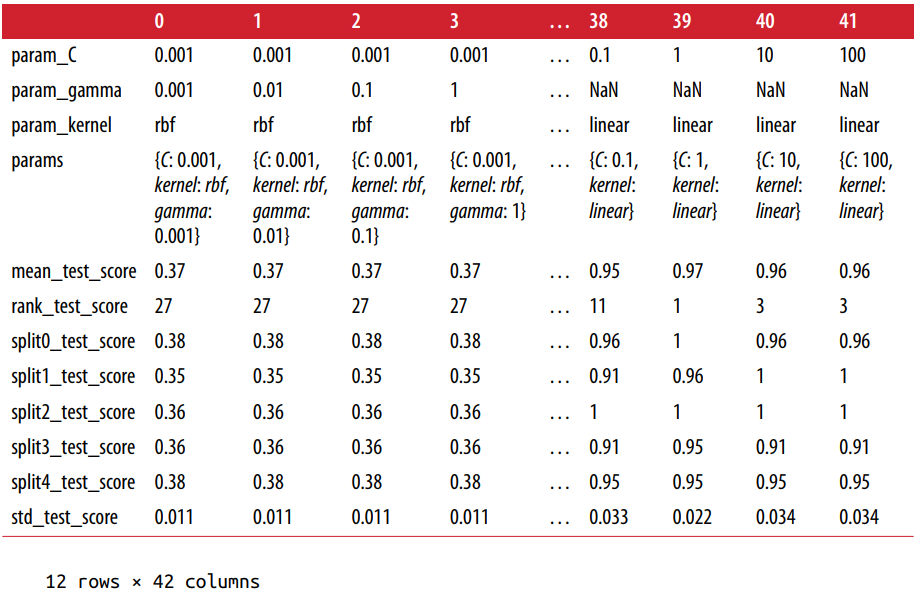
\includegraphics[scale=0.7]{Imagen_Machine/DataGrid}
	%\caption{Matriz de confusión para clasificación binaria}
	\label{DataGrid}
\end{figure}

\newpage


\subsubsection{Uso de diferentes estrategias de validación cruzada con  grid search}

De forma similar a {\ttfamily cross\_val\_score,  GridSearchCV} utiliza validación cruzada estratificada de k-fold por defecto para la clasificación y validación cruzada k-fold para la regresión.  Sin embargo, usted también puede pasar o agregar cambios a cualquier divisor de validación cruzada, como se describe en la sección \ref{VC} en la página \pageref*{VC}, como el parámetro {\ttfamily cv} en {\ttfamily GridSearchCV}. En particular, para obtener sólo una única división en un conjunto de entrenamiento y validación, se  puede usar  {\ttfamily ShuffleSplit o StratifiedShuffleSplit} con {\ttfamily n\_iter = 1}. Esto podría ser útil para datas muy grandes o modelos muy lentos.


{\subsubsection{Validación cruzada anidada}


En los ejemplos anteriores, pasamos de usar una simple  división de datos en entrenamiento,
validación y pruebas, a dividir los datos del entrenamiento y pruebas, para luego realizar la validación cruzada en el conjunto de entrenamiento. 

Pero al usar GridSearchCV  descrito anteriormente, todavía tenemos una sola división de los datos en conjuntos de entrenamiento y prueba,
lo que podría hacer que nuestros resultados sean inestables y hacernos depender demasiado de esta única división de los datos. 

Pero al usar {\ttfamily GridSearchCV} como se describió anteriormente, todavía tenemos una sola división de los datos en el conjuntos de entrenamiento y pruebas, lo que podría hacer que nuestros resultados sean inestables y hacernos depender demasiado de esta única división de los datos.

Podemos ir un paso más allá y, en lugar de dividir los datos originales en los conjuntos 
de entrenamiento y prueba una vez, use múltiples divisiones de validación cruzada. 
Esto resultará en lo que se llama validación cruzada anidada.

En la validación cruzada anidada, hay un bucle exterior sobre divisiones  de los datos en conjuntos de entrenamiento y prueba. Para cada uno de ellos, se ejecuta  una búsqueda de cuadrícula  (grid search)
(lo que puede dar como resultado mejores parámetros  diferentes  para cada división en el bucle exterior).    Luego, para cada división externa, se usa el  mejor  score  puntuación del conjunto de pruebas para la  configuración. \\

Los resultados de este procedimiento es una lista de puntajes, no es un modelo y ni un conjunto de parámetros.   Los puntajes nos dicen qué tan bien generaliza un modelo, dados los mejores parámetros encontrados  por la cuadrícula.


Como no proporciona un modelo que se pueda usar en datos nuevos, la validación cruzada anidada rara vez se usa cuando se busca un modelo predictivo para aplicar a datos futuros.
Sin embargo, puede ser útil para evaluar qué tan bien funciona un modelo dado en una data particular. 

Implementar la validación cruzada anidada en {\ttfamily scikit-learn} es sencillo.  Llamando {\ttfamily 
cross\_val\_score} con una instancia de {\ttfamily GridSearchCV} como modelo:


\begin{lstlisting}%[frame=single]

In[34]:
   
   scores = cross_val_score(GridSearchCV(SVC(), param_grid, cv=5),
                            iris.data, iris.target, cv=5)
   print("Cross-validation scores: ", scores)
   print("Mean cross-validation score: ", scores.mean())

Out[34]:

    Cross-validation scores: [ 0.967 1. 0.967 0.967 1. ]
    Mean cross-validation score: 0.98

\end{lstlisting}


El resultado de esta validación cruzada anidada se puede resumir como un modelo "{}SVC 
que puede alcanzar el 98\%  exactitud media de validación cruzada en el conjunto de
datos del iris{}"{},  nada más y nada Menos.\\

Aquí, utilizamos validación cruzada estratificada de 5-fold  tanto en el bucle interior como en el exterior. Como el {\ttfamily param\_grid} contiene 36 combinaciones de parámetros,   esto da como resultado un la enorme cantidad de  36 * 5 * 5 =  900  modelos en construcción,  lo que hace que la validación cruzada anidada sea un procedimiento muy costoso.    Aquí, utilizamos la  misma división  de validación cruzada en el bucle interior y en el externo; sin embargo, esto no es necesario y puede usar cualquier combinación
de estrategias de validación cruzada en los bucles interno y externo.

Esto puede ser un poco complicado para entender lo que está sucediendo en la simple línea  dada anteriormente, y puede ser útil visualísarlo  por bucles, como se hace en la siguiente implementación simplificada:


\begin{lstlisting}%[frame=single]

In[35]:

   def nested_cv(X, y, inner_cv, outer_cv, Classifier, parameter_grid):
       outer_scores = []
       # for each split of the data in the outer cross-validation
       # (split method returns indices)
       for training_samples, test_samples in outer_cv.split(X, y):
           # find best parameter using inner cross-validation
           best_parms = {}
           best_score = -np.inf
           # iterate over parameters
           for parameters in parameter_grid:
               # accumulate score over inner splits
               cv_scores = []
               # iterate over inner cross-validation
               for inner_train, inner_test in inner_cv.split(
                       X[training_samples], y[training_samples]):
                   # build classifier given parameters and training data
                   clf = Classifier(**parameters)
                   clf.fit(X[inner_train], y[inner_train])
                   # evaluate on inner test set
                   score = clf.score(X[inner_test], y[inner_test])
                   cv_scores.append(score)
               # compute mean score over inner folds
               mean_score = np.mean(cv_scores)
               if mean_score > best_score:
                  # if better than so far, remember parameters
                  best_score = mean_score
                  best_params = parameters
          # build classifier on best parameters using outer training set
          clf = Classifier(**best_params)
          clf.fit(X[training_samples], y[training_samples])
          # evaluate
          outer_scores.append(clf.score(X[test_samples], y[test_samples]))
       return np.array(outer_scores)

\end{lstlisting}

Ahora, vamos a correr  esta función sobre la data iris: 

\begin{lstlisting}%[frame=single]

In[36]:
   
   from sklearn.model_selection import ParameterGrid, StratifiedKFold
   scores = nested_cv(iris.data, iris.target, StratifiedKFold(5),
                      StratifiedKFold(5), SVC, ParameterGrid(param_grid))
   print("Cross-validation scores: {}".format(scores))

Out[36]:
    
    Cross-validation scores: [ 0.967 1. 0.967 0.967 1. ]

\end{lstlisting}


\subsection{Paralelismos entre validación cruzada y búsqueda de cuadrícula}
 % embarrassingly
 
Mientras se ejecuta una grid search  sobre muchos parámetros y en una data grande 
puede ser un gran reto computacionalmente y hasta difícil, también es paralelamente enrredado. 
Esto significa que construir   un modelo usando una configuración  particular de parámetro con  una división de validación cruzada específica, se puede desarrollarse completamente independientemente de las otras configuraciones de parámetros y modelos. 

Esto hace que  la grid search  búsqueda de cuadrícula y la validación cruzada sean candidatos ideales para la paralelización sobre múltiples núcleos (cores) de CPU o sobre un clúster. Puede utilizar varios núcleos en  {\ttfamily GridSearchCV} y {\ttfamily cross\_val\_score} para configurar  el parámetro
  {\ttfamily n\_jobs} como el número de núcleos de CPU que quiere usar. Puede configurar 
  {\ttfamily n\_jobs=-1} para usar todos los núcleos disponibles.



Debe tener en cuenta que {\ttfamily scikit-learn}  {\bf no permite} anidar operaciones paralelas.
Así, que si está utilizando la opción {\ttfamily n\_jobs} en su modelo (por ejemplo, un bosque aleatorio),
no puede usarlo en {\ttfamily GridSearchCV} para busquedas sobre  este modelo. 
Si la  data y el modelo son muy grande, puede que usar muchos cores núcleos que  consumen  demasiada memoria,
y debe monitorear su uso de la memoria al construir modelos grandes en paralelo.\\

También es posible paralelizar la   búsqueda de cuadrícula (grid search) y la validación cruzada en varias
máquinas en un clúster, aunque al momento de escribir esto no hay  compatible con {\ttfamily scikit-learn}.
Sin embargo, es posible utilizar el marco de trabajo de IPython en paralelo  para   búsquedas de cuadrícula paralelas, si no se le facilita  escribir el bucle  sobre los parámetros como lo hicimos 
en sección \ref{Gsear} en la página  \pageref*{Gsear}.\\

Para los usuarios de {\ttfamily   Spark}, también existe el paquete   \href{https://github.com/databricks/spark-sklearn}{\textcolor{vino}{\ttfamily spark-sklearn}}  desarrollado recientemente, que permite ejecutar una  grid search  en un clúster Spark ya establecido.







\section{Métricas de evaluación y puntuación}

Hasta ahora, hemos evaluado el rendimiento de clasificación utilizando la exactitud (accuracy) la fracción de muestras clasificadas correctamente  y el rendimiento de regresión utilizando $R^{2}$. 
 Sin embargo, estos son sólo dos de las tanta formas posibles de resumir qué tan bien funciona un modelo supervisado en una  dataset dada. En la práctica, estas métricas de evaluación pueden no ser apropiadas  para su aplicación, y es importante elegir la métrica correcta al seleccionar entre modelos y parámetros de ajuste.


\subsubsection{Mantenga el objetivo final en presente}

Al seleccionar una métrica, siempre debe tener encuenta el objetivo final de la aplicación  del aprendizaje automático.  En la práctica, generalmente estamos interesados no sólo en hacer predicciones exactas, sino tanbien en  usar estas predicciones como parte de un proceso de toma de decisiones más amplio. Antes de elegir una métrica de aprendizaje automático, debe pensar en el objetivo del alto nivel de la aplicación, a menudo denominado \emph{métrica empresarial} (business metric).   Las  consecuencias de elegir un algoritmo particular para una aplicación de aprendizaje automático se denominan {\ttfamily impacto empresarial}\footnote{\scriptsize	  Pedimos a los lectores con tendencia científica que disculpen el lenguaje comercial en esta sección. No perder de vista el objetivo final es igualmente importante en la ciencia, aunque los autores no son conscientes de una frase similar a "{}impacto empresarial"{} que se utiliza en ese ámbito.}   %    called the business metric. 

Tal vez el objetivo de alto nivel es evitar accidentes de tránsito, o disminuir el número de 
ingresos hospitalarios. También podría ser obtener más usuarios para el sitio web, o hacer
 que los usuarios gasten más dinero en su tienda.   Al elegir un  modelo o ajuste de 
 parámetros, debe elegir los valores del modelo o parámetro que más influencia más positiva 
 genera  en la métrica empresarial.  Generalmente esta tarea es difícil, ya que evaluar el impacto empresarial de un modelo en particular podría requerir ponerlo en producción en un sistema de la vida real.\\


En las primeras etapas del desarrollo, y mientras se ajustan los parámetros, generalmente no es viable
 poner el modelo en producción sólo con el próposito de prueba, debido a la alta actividad comercial
o riesgos personales que pueden estar involucrados. 

Por lo tanto, a menudo necesitamos encontrar algún procedimiento de evaluación sustituto, utilizando una métrica de evaluación que sea más fácil de calcular. \\

Escribir introducción a al objetivo de la metrica modelo\\

% Imagine evaluating the pedestrian avoidance capabilities of a self-driving car by just letting it drive around, without verifying it first; if your model is bad, pedestrians will be in trouble! Therefore we often need to find some surrogate evaluation procedure, using an evaluation metric that is easier to compute. For example, we could test classifying images of pedestrians against nonpedestrians and measure accuracy. Keep in mind that this is only a surrogate, and it pays off to find the closest metric to the original business goal that is feasible to evaluate. This closest metric should be used whenever possible for model evaluation and selection. The result of this evaluation might not be a single number—the conse‐quence of your algorithm could be that you have 10\% more customers, but each customer will spend 15\% less  —but it should capture the expected business impact of choosing one model over another.\\ Por ejemplo, podríamos probar la clasificación de imágenes de peatones contra no peatones y medir la exactitud (accuracy). Tenga en cuenta que esto es sólo un sustituto, y vale la pena encontrar la métrica más cercana al objetivo comercial original que sea factible de evaluar.  Esta métrica más cercana debe usarse siempre que sea posible para la evaluación  y selección  del modelo.   El resultado de esta evaluación podría no ser un simple número: la consecuencia  del algoritmo podría ser que tienes un 10\% más de clientes,  cada cliente gastará un 15\% menos,  debería capturar el impacto comercial esperado al elegir un modelo sobre otro.\\


En esta sección, primero discutiremos las métricas para el caso especial importante de la
clasificación  binaria, luego volvemos  a la clasificación multiclase y finalmente a la  regresión.

\subsection{Métricas para la clasificación binaria}

La clasificación binaria es posiblemente la aplicación más común y conceptualmente la aplicación más simple del aprendizaje automático en la práctica.  Sin embargo, todavía hay una serie de advertencias en la evalualuación incluso en esta  tarea simple.   Antes de sumergirnos en métricas alternativas, veamos  las formas en que la medición de la exactitud (accuracy) puede ser engañosa. Recuerda que para la clasificación binaria, frecuentemente  hablamos de una clase positiva y una clase negativa,  entendiendose que la clase positiva es la que estamos buscando.


\subsection{Tipos de errores}

Generalmente  la exactitud (accuracy) no es una buena medida del rendimiento predictivo, ya que el número de
los errores que cometemos no contienen toda la información que nos interesa. Imagine
una aplicación de pantalla para la detección anticipada de cáncer mediante una prueba automatizada. 
Si la prueba es negativa, se supondrá que el paciente está sano, mientras que si la prueba es positiva, 
el paciente se someterá a una evaluación adicional.   Aquí, llamaríamos a la prueba positiva 
(una indicación  de cáncer) como la clase positiva, y una prueba negativa a la clase negativa. No podemos
asumir que el modelo siempre funcionará perfectamente, es decir cometerá errores. Para cualquier
aplicación, debemos preguntarnos cuáles podrían ser las consecuencias de estos errores 
en el mundo real.\\

Un posible error podría ser que  un paciente sano sea clasificado como positivo, lo que lleva a
pruebas adicionales.  Esto genera  algunos costos e inconveniente para el paciente (posiblemente algo de angustia mental).  Una predicción positiva incorrecta se llama un \emph{falsa positivo}. El otro posible error ocurre cuando un paciente enfermo es clasificado como negativo, y en consecuencia no recibirá más pruebas y ni tratamiento. El cáncer no diagnosticado puede conducir a problemas de  graves de salud, e incluso podrían ser fatales.   Un error de este tipo, una precición   negativa  incorrecta: se llama  \emph{falso negativo}.   

En estadística, un \emph{falso positivo} es conocido como \emph{error tipo I}, y un \emph{falso negativo} es conocido como \emph{ error tipo II}.  Nos apegaremos  al   “{}falso positivo"{} y al "falso negativo”,  ya que son más explícitos y más fáciles de recordar. \\

En el ejemplo de diagnóstico de cáncer, es claro que queramos evitar \emph{falsos negativas} en lo más posible, mientras los falsos positivos pueden ser vistos como de una molestia menor.  Si bien este es un ejemplo particularmente drástico, la consecuencia de falsos positivos y los falsos negativos rara vez son iguales.   En aplicaciones comerciales, podría ser posible asignar valores en dólares en ambos 
tipos de errores, lo que permitiría medir el error de una predicción particular en 
dólares, en lugar de exactitud (accuracy). Esto podría ser mucho más significativo para tomar 
decisiones comerciales respecto a qué modelo utilizar.


\subsection{Datas desbalanceadas}


%  El desbalanceo de clases aparece en entornos variados como pueden ser la detección de fraude, enfermedades o spam.

Los tipos de errores juegan un papel importante cuando una de dos clases es mucho más frecuente
que el otro.  Esto es muy común en la práctica;  un buen ejemplo es la predicción de clics, donde cada punto de dato representa una "{}impresión"{}, un item que fue  mostrado al  usuario.   Este item  puede ser un anuncio, una historia relacionada o una persona a seguir en una red social. El objetivo es predecir si  se muestra un item en particular, un usuario hará clic en él (indicando que está interesado). La mayoría de las cosas que se muestran en Internet (en particular, los anuncios) no generará un clic. Es posible que deba mostrar a un usuario 100 anuncios o artículos antes de que encuentren algo lo suficientemente interesante como para hacer clic.  Esto da como resultado una data  donde por cada 99 puntos de datos "{}sin clic"{}, hay un dato  "{}cliqueados"{}; en otras palabras, el 99\% de las muestras pertenecen a la clase "{}sin clic"{}.  Una Data en cuál una  clase es mucho más frecuente que la otra, se llama desbalanceada,  o data con clases desbalanceada.  En realidad,  las datas desbalanceada es lo más común, y es raro que los eventos de interés tengan una frecuencia igual o incluso similar en la data.\\

Ahora supongamos que construimos  un clasificador con una exactitud (accuracy) del 99\% en la tarea de  predicción de clics.  ¿Qué te dice eso?  99\%  de  exactitud (accuracy) suena impresionante,  pero esto no toma en cuenta el desbalance  de clase, o de la data. Puede lograr una  exactitud (accuracy)  del 99\% sin construir un modelo de aprendizaje automático, pues al predecir siempre será  "{}sin clic"{}. 

Por otro lado, incluso con datos desbalanceados, un modelo con una exactitud (accuracy) del 99\% podría ser bastante bueno.   Sin embargo, la exactitud (accuracy) no nos permite distinguir la  constante  "{}sin clic"{}  de un modelo potencialmente  bueno.\\

Para ilustrarlo, creamos un conjunto de datos desbalanceados  9: 1,  a partir de la dataset  dígitos, por clasificación el dígito 9 contra las otras nueve clases:

   
\begin{lstlisting}%[frame=single]

In[37]:

   from sklearn.datasets import load_digits
   
   digits = load_digits()
   y = digits.target == 9
   
   X_train, X_test, y_train, y_test = train_test_split(
        digits.data, y, random_state=0)

\end{lstlisting}


Podemos usar el {\ttfamily DummyClassifier} para predecir siempre la clase mayoritaria (aquí "{}no nueve"{}) para ver cómo  puede  desinformar la  exactitud (accuracy):

\begin{lstlisting}%[frame=single]

In[38]:
   
   from sklearn.dummy import DummyClassifier
   dummy_majority = DummyClassifier(
            strategy='most_frequent').fit(X_train, y_train)
   pred_most_frequent = dummy_majority.predict(X_test)
   print("Unique predicted labels: {}".format(np.unique(pred_most_frequent)))
   print("Test score: {:.2f}".format(dummy_majority.score(X_test, y_test)))

Out[38]:
   
    Unique predicted labels: [False]
    Test score: 0.90

\end{lstlisting}

Obtuvimos una  exactitud (accuracy) cercana al 90\% sin aprender nada. Esto puede parecer llamativo, pero piénselo por un minuto. Imagina que alguien te dice que su modelo es 90\%  exacto (accuracy). Se podría pensar que hicieron un  buen trabajo. Pero dependiendo del problema, ¡eso podría ser posible prediciendo  simplemente  una clase! 

Comparemos  esto   con resultado de un clasificador real:

\begin{lstlisting}%[frame=single]

In[39]:

   from sklearn.tree import DecisionTreeClassifier
   tree = DecisionTreeClassifier(max_depth=2).fit(X_train, y_train)
   pred_tree = tree.predict(X_test)
   print("Test score: {:.2f}".format(tree.score(X_test, y_test)))

Out[39]:
   
   Test score: 0.92

\end{lstlisting}



Según la  exactitud (accuracy), el clasificador {\ttfamily DecisionTreeClassifier} es sólo un poco mejor que el predictor constante. Esto podría indicar que algo está mal con la forma en que
utilizó el clasificador  {\ttfamily DecisionTreeClassifier}, o esa medidad de exactitud aquí no es una buena.\\


Para própositos  de comparación, evalúemos dos clasificadores más, el {\ttfamily LogisticRegression}
y el {\ttfamily DummyClassifier} por defecto, que realiza predicciones aleatorias pero produce
clases con las mismas proporciones que las del conjunto de entrenamiento:


\begin{lstlisting}%[frame=single]

In[40]:
   
   from sklearn.linear_model import LogisticRegression
   
   dummy = DummyClassifier().fit(X_train, y_train)
   pred_dummy = dummy.predict(X_test)
   
   print("dummy score: {:.2f}".format(dummy.score(X_test, y_test)))
   logreg = LogisticRegression(C=0.1).fit(X_train, y_train)
   pred_logreg = logreg.predict(X_test)
   print("logreg score: {:.2f}".format(logreg.score(X_test, y_test)))

Out[40]:

   dummy score: 0.80
   logreg score: 0.98
   
\end{lstlisting}

El clasificador dummy que produce resultados aleatorios es claramente el peor los demás (según la  exactitud), mientras que {\ttfamily LogisticRegression} produce muy buenos resultados.
Sin embargo, incluso el clasificador aleatorio produce más del 80\% de  exactitud (accuracy). Esto  hace muy
 difícil juzgar cuál de estos resultados es realmente útil. El problema aquí es que la  exactitud (accuracy)  es una medida inadecuada para cuantificar el rendimiento predictivo en esta data desbalanceado.

Para el resto de este capítulo, exploraremos métricas alternativas que proporcionar una mejor orientación en la selección de modelos. En particular, nos gustaría tener métricas  que nos indiquen qué tan bueno es un modelo para  hacer predicciones  "{}más frecuentes"{}  o  predicciones aleatorias, como ellas son  calculadas   en { \ttfamily pred\_most\_frequent}  y  {\ttfamily pred\_dummy}.
 Si utilizamos una métrica para evaluar nuestros modelos, definitivamente debería ser capaz de
eliminar estas predicciones sin sentido.


\subsection{Matrices de confusión} 

Una de las formas más completas de representar el resultado de la evaluación de una clasificación 
binaria es utilizando matrices de confusión.  

Inspeccionemos las predicciones de {\ttfamily LogisticRegression} de la sección anterior usando 
 la función  {\ttfamily confusion\_matrix};   las predicciones sobre el conjunto de  pruebas  ya estan almacenadas en  {\ttfamily pred\_logreg}:


\begin{lstlisting}%[frame=single]

In[41]:

   from sklearn.metrics import confusion_matrix
   confusion = confusion_matrix(y_test, pred_logreg)
   print("Confusion matrix:\n{}".format(confusion))

Out[41]:
    
     Confusion matrix:
     [[401 2]
      [ 8 39]]
     
\end{lstlisting}


La salida de {\ttfamily confusion\_matrix} es un arreglo  2x2,  donde las filas corresponden
a las  verdaderas   clases  y las columnas concuerda con la predición de clases.    Cada  entrada cuenta la frecuencia con que una muestra que pertenece a la clase correspondiente en la fila  (en este caso es  "{}no nueve"{} y "{}nueve{}") es clasificada como la clase correspondiente en la columna.


El siguiente gráfico  (la Figura \ref{Confusion}) ilustra esta descripción:

\begin{lstlisting}%[frame=single]

In[42]:

   mglearn.plots.plot_confusion_matrix_illustration()

\end{lstlisting}


\begin{figure}[h!]
	\centering
	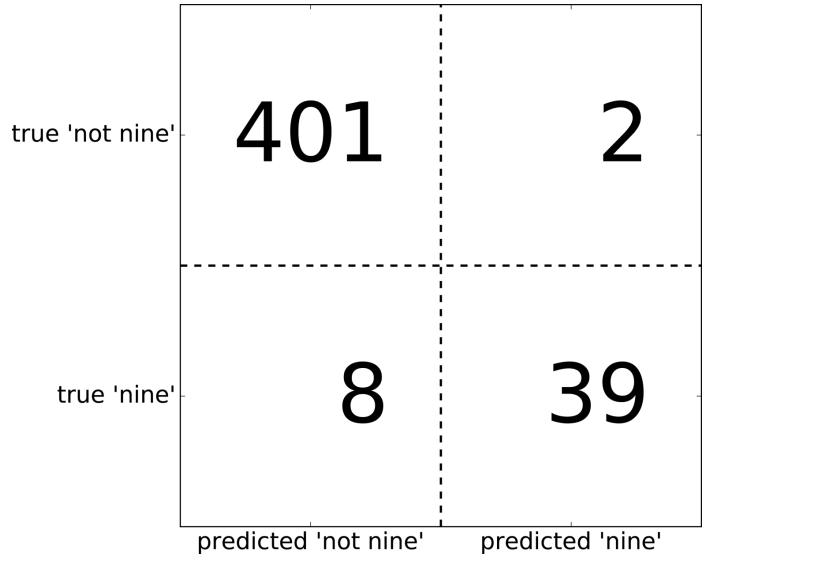
\includegraphics[scale=0.55]{Imagen_Machine/Confusion}
	\caption{Matriz de confusión de la tarea de clasificación "{}nueve vs. resto"{}}
	\label{Confusion}
\end{figure}

Las entradas en la diagonal principal\footnote{\scriptsize	  La diagonal principal de una matriz bidimensional o matriz A es A[i, i].} de la matriz de confusión corresponden a la clasificación correcta, mientras que otras entradas nos dicen cuántas muestras de una clase se clasificaron  erróneamente  como otra clase.\\

Si declaramos "{}un nueve"{} como clase positiva, podemos relacionar las entradas de la matriz de 
 confusión   con los términos falso positivo y falso negativo que presentamos anteriormente. 

Para completar el cuadro, llamamos  a las muestras clasificadas  correctamente  pertenecientes
a la clase positiva como  verdadera positiva  (true positives), y  a las muestras 
clasificadas correctamente   pertenecientes a la clase negativa como  verdadero negativos  (true negatives).
Estos términos generalmente se abrevian FP, FN, TP y TN  y  conducen a la siguiente
interpretación de  la matriz de confusión (Figura \ref{Confusion2}):





\begin{lstlisting}%[frame=single]

In[43]:

   mglearn.plots.plot_binary_confusion_matrix()

\end{lstlisting}


\begin{figure}[h!]
	\centering
	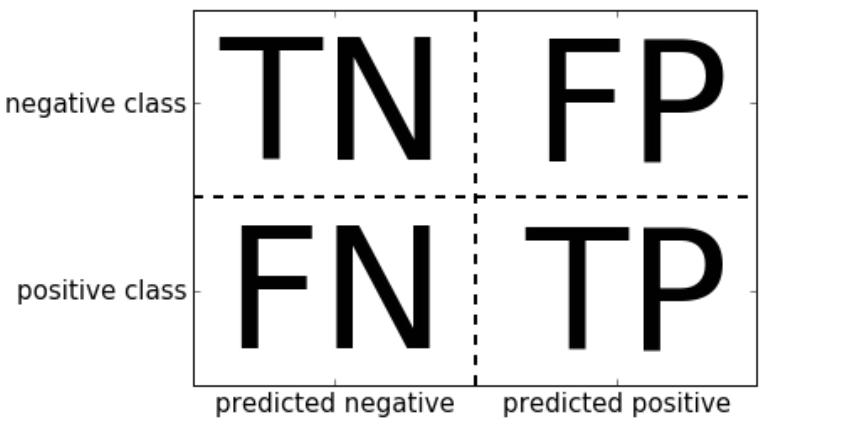
\includegraphics[scale=0.55]{Imagen_Machine/Confusion2}
	\caption{Matriz de confusión para clasificación binaria}
	\label{Confusion2}
\end{figure}



Ahora usemos la matriz de confusión para comparar los dos modelos que ajustamos anteriormente 
(los modelos simulados por  árbol de decisión y  por regresión logística):


\begin{lstlisting}%[frame=single]

In[44]:

   print("Most frequent class:")
   print(confusion_matrix(y_test, pred_most_frequent))
   print("\nDummy model:")
   print(confusion_matrix(y_test, pred_dummy))
   print("\nDecision tree:")
   print(confusion_matrix(y_test, pred_tree))
   print("\nLogistic Regression")
   print(confusion_matrix(y_test, pred_logreg))

Out[44]:

   Most frequent class:
   [[403 0]
    [ 47 0]]
   Dummy model:
   [[361 42]
    [ 43 4]]
   Decision tree:
   [[390 13]
    [ 24 23]]
   Logistic Regression
   [[401 2]
    [ 8 39]]

\end{lstlisting}


Observando la matriz de confusión, es bastante claro que algo está mal con
{\ttfamily pred\_most\_frequent}, porque siempre predice la misma clase (negativa). 
Por otro lado,  {\ttfamily pred\_dummy}  tiene un número muy pequeño de 
 verdaderos positivos  (4), que particularmente en comparación con
la cantidad de falsos negativos y falsos positivos:  hay muchos más falsos positivos
que  verdaderos positivos!   Las predicciones hechas por el árbol de decisión tienen  mucho más
sentido que las predicciones dummy, a pesar de que la exactitud era casi la misma. 
Finalmente, podemos ver que la regresión logística funciona mejor que  {\ttfamily pred\_tree} en todos los aspectos: tiene más verdaderos positivos   y  verdaderos  negativos,  y   pocos  falsos positivos y falsos negativos.    De esta comparación, está claro que sólo el árbol de decisión y la logística
la regresión da resultados razonables, y la regresión logística funciona mejor que
el árbol en todas las cuentas. 


Sin embargo, inspeccionar la matriz de confusión completa es un poco engorroso,
y aunque  ganamos   gran cantidad de información al observar todos los aspectos de la matriz,
el proceso fue muy manual y cualitativo.  Hay varias formas de resumir la información en la matriz de confusión, que discutiremos a continuación.


\subsection{Relación con la exactitud (Accuracy).} 

 Ya vimos una forma de resumir el resultado en  la matriz de confusión: calculando la exactitud,  se puede expresar como:\\

$ \text{Accuracy} = \text{exactitud} = \frac{TP+TN}{TP + TN + FP + FN} $\\


En otras palabras, la exactitud (Acuracy) es el número de predicciones correctas (TP y TN) divididas
por el número de total de las muestras (todas las entradas de la matriz de confusión resumidas).

\subsection{Precisión, Sensibilidad y f-puntuación\\ (en Inglés Precision, recall, and f-score)}
	
%	Recall =  sensitivity      %    también llamado  Tasa de Verdaderos Positivos 
 
 Hay varias otras formas de resumir la  matriz confusión, siendo unas de las más comunes la \emph{precisión} (en inglés precision)  y  la \emph{sensibilidad} (en Inglés Recall o sensitivity).\\  
 
 La  precisión  mide cuántas muestras predichas como positivas son realmente positivas:\\

$\text{Precision} =  \text{Precisión} = \frac{TP}{TP +  FP} $  \\  %  TP   TP+FP

          
La  precisión se utiliza como una métrica de rendimiento cuando el objetivo es limitar el número de falsos positivos.   Como ejemplo, imagine un modelo para predecir si un nuevo medicamento será eficaz en el tratamiento de una enfermedad en ensayos clínicos.   Por lo general los ensayos clínicos son notoriamente  costosos, y una compañía farmacéutica   solo querrá realizar un experimento si es  muy seguro de que la droga
  realmente funcionará.  Por lo tanto, es importante que el modelo no produzca muchos falsos positivos, en otras palabras, que tenga  alta precisión.   La precisión  también se conoce como    \emph{ valor predictivo positivo} (VPP).\\
 
Por otro lado,  la sensibilidad (en Inglés Recall o sensitivity),  mide cuántas de las muestras positivas son capturadas  por las predicciones positivas:\\

$ \text{Recall} = \text{sensibilidad} = \frac{TP}{TP +  FN} $  \\   %  TP   TP+FN  


La sensibilidad se utiliza como medida de rendimiento cuando necesitamos identificar todas las muestras positivas; es decir, cuando es importante evitar falsos negativos. El ejemplo del diagnóstico de cáncer dado en este capítulo, es un buen ejemplo de este caso: es importante encontrar todas las personas que están enfermas, posiblemente incluyendo  pacientes sanos en la predicción. 

Otros nombres dados a Recall son sensibilidad  o exhaustividad, \emph{tasa de éxito, o tasa de Verdaderos Positivos} (TPR).\\

Hay  una compensación entre optimizar la sensibilidad y optimizar la precisión. 
Puedes trivialmente   obtener una sensibilidad perfecta si predice que todas las muestras  que pertenecen a la clase positiva: no habrá falsos negativos y ni tampoco verdaderos negativos.   Sin embargo, prediciendo todas las muestras como  positivas darán como resultado muchos falsos
 positivos, y por lo tanto, la  precisión  debe ser muy bajo.    Por otro lado, 
 si  encuentra un modelo que predice sólo los datos individuales que son más seguros de ser positivos y 
  el resto como negativo, entonces la precisión  será perfecta (asumiendo que este punto es de hecho positivo), pero la sensibilidad será muy mala.\\


\begin{minipage}[t]{0.2\textwidth}
	\centering\raisebox{\dimexpr \topskip-\height}{%
		
\includegraphics[width=\textwidth]{Imagen_Machine/Zorrillo}}
\end{minipage}%\hfill
\begin{minipage}[t]{0.75\textwidth} 
	{\scriptsize
	La precisión y la sensibilidad son sólo dos de las tantas medidas de clasificación derivadas de TP, FP, TN y FN. Puedes encontrar un gran resumen de todas las medidas en   \href{https://en.wikipedia.org/wiki/Sensitivity_and_specificity}{\textcolor{vino}{Wikipedia} }. En la comunidad de aprendizaje automático, la precisión  y la sensibilidad son sin duda las medidas más utilizadas para la clasificación binaria, pero otras comunidades podrían utilizar otras métricas relacionadas.}
\end{minipage}\\




Si bien,  la precisión y la sensibilidad son medidas muy importantes, observar una sóla  de
ellas no le proporcionarán la imagen completa de la situación.   Una forma de resumirlos es la métrica  {\ttfamily f-score}  o  {\ttfamily f-measure},  que tiene la media armónica de la  precisión y la  sensibilidad: \\

$ F = 2 \cdot \frac{\text{ precisión} \cdot \text{sensibilidad}}{\text{ precisión}
	 + \text{sensibilidad}}  $ \\

Esta variante particular también se conoce como $f_{}1$ -puntuación  ($f_{1}$-score).  Como métrica que  toma en cuenta  la  precisión y la sensibilidad, puede ser una mejor medida que la exactitud  (accuracy) en la clasificación binaria con  data desbalanceada. 

Vamos a correr esta métrica sobre las predicciones de la data  "{}nueve vs. resto"{},  que 
se calculó  anteriormente.  Aquí, asumiremos que el "{}nueve"{} es la clase positiva (etiquetado como verdadero mientras que el resto está etiquetado como falso), por lo que la clase positiva es la clase de la minoritaria:  

\begin{lstlisting}%[frame=single]

In[45]:

   from sklearn.metrics import f1_score
   print("f1 score most frequent: {:.2f}".format(
           f1_score(y_test, pred_most_frequent)))
   print("f1 score dummy: {:.2f}".format(f1_score(y_test, pred_dummy)))
   print("f1 score tree: {:.2f}".format(f1_score(y_test, pred_tree)))
   print("f1 score logistic regression: {:.2f}".format(
           f1_score(y_test, pred_logreg)))

Out[45]:

   f1 score most frequent: 0.00
   f1 score dummy: 0.10
   f1 score tree: 0.55
   f1 score logistic regression: 0.89

\end{lstlisting}


Podemos notar dos cosas aquí. Primero, recibimos un mensaje de error para  la predicción de  {\ttfamily most\_frequent}, ya que no hubo predicciones de la clase positiva (lo que hace que el
denominador de $f$-puntuación sea cero ($f$-score)).   Además, podemos ver una distinción bastante fuerte entre
las predicciones de dummy  y las predicciones de árbol, que no estaban claras al trabajar con la
exactitud (accuracy) por sí sola. 
Usando la $f$-puntuación ($f$-score)  para la evaluación, resumimos el rendimiento predictivo de nuevo en un número.  Sin embargo, la $f$-puntuación  parece capturar nuestra intuición, de qué hace  un buen modelo mucho mejor de lo que la exactitud (accuracy) lo hizo.   No obstante, una desventaja de la $f$-puntuación,  es que es más difícil de interpretar y explicar que la exactitud.\\
 
 
Por otro lado, si se quiere un resumen más completo de las medidas de exactitud, sensibilidad y  $f$-puntaje,   puede usar la función de conveniencia {\ttfamily classification\_report}  para calcular los tres a la vez, e imprimirlos en un formato agradable:

\begin{lstlisting}%[frame=single]

In[46]:

   from sklearn.metrics import classification_report
   print(classification_report(y_test, pred_most_frequent,
                               target_names=["not nine", "nine"]))

Out[46]:

            precision   recall   f1-score  support
             
   not nine     0.90      1.00       0.94      403
   nine         0.00      0.00       0.00       47
   
   avg / total  0.80      0.90       0.85      450



\end{lstlisting}



La función {\ttfamily classification\_report} produce una línea por clase (aquí, True y False) y reporta precisión, sensibilidad y $f$-puntuación con esta clase como la clase positiva. Antes, asumimos que la clase  minoritaria "{}nueve"{}  era la clase positiva.  Si cambiamos la clase positiva a "{}no nueve"{},  podemos ver en la salida de {\ttfamily  classification\_report}  un $f$-puntaje de 0.94 para el modelo {\ttfamily most\_frequent}.  Además, para la clase "{}no nueve"{} \: tenemos una sensibilidad de 1, ya que clasificamos todas las muestras como  "{}no nueve."{}    La última columna junto a la $f$-puntuación proporciona el soporte de cada clase, lo que simplemente significa el número de muestras en esta clase de acuerdo a la verdad fundamental.\\


 
La última fila del informe de clasificación muestra una ponderación (por el número de muestras
en la clase) promedio de los números por cada clase.  Aquí hay dos informes o reportes más, uno para
el clasificador dummy y otro para la regresión logística:


\begin{lstlisting}%[frame=single]

In[47]:

   print(classification_report(y_test, pred_dummy,
                               target_names=["not nine", "nine"]))

Out[47]:

              precision    recall   f1-score   support
      
    not nine       0.90      0.92       0.91       403
       nine        0.11      0.09       0.10        47

   avg / total     0.81      0.83       0.82       450 

In[48]:

   print(classification_report(y_test, pred_logreg,
                               target_names=["not nine", "nine"]))

Out[48]:

              precision    recall   f1-score   support

   not nine        0.98      1.00        0.99      403
       nine        0.95      0.83        0.89       47

  avg / total      0.98      0.98        0.98      450


\end{lstlisting}

Como puede notar al observar los reportes, las diferencias entre el modelo dummy
y un buen modelo ya no son tan claros.  La elección de qué clase es declarada como la clase positiva tiene un gran impacto en las métricas.  Mientras que la $f$-puntuación para la clasificación dummy es 0.10  (vs. 0.89 para la regresión logística) en la clase "{}nueve"{}, para la clase "{}no nueve"{}  es 0.91 vs. 0.99, que parecen resultados razonables.  Sin embargo, al observar todos los números juntos pinta una imagen bastante exacta (accuracy), y podemos ver claramente la superioridad del modelo de regresión logística.

\subsection{Tomando en cuenta la incertidumbre}

La matriz de confusión y el reporte de clasificación proporcionan un análisis  detallado de
un conjunto particular de predicciones. Sin embargo,  las propias predicciones  ya arrojaron
una gran cantidad de información contenida en el modelo.   Como discutimos en el capítulo \ref{Cap2}, la mayoría de los clasificadores proporcionan un método  {\ttfamily decision\_function}  o  {\ttfamily predict\_proba }  para  evaluar el grado de certeza sobre las predicciones.  Hacer predicciones puede verse como un  umbral de la salida de {\ttfamily decision\_function}  o  {\tt predict\_proba }  en un cierto punto fijo; en la clasificación binaria usamos 0  para la función de decisión y  0.5  para  {\ttfamily predict\_prob}.\\

 
 A continuación se presenta un ejemplo de una tarea de clasificación binaria sobre una data desbalanceada, con 400  puntos clasificados  en la clase negativa contra 50 puntos en la clase positiva.  
 Los datos de entrenamiento se muestran a la izquierda en la Figura \ref{Impacto}. Se entrena  un modelo SVM kernel  sobre estos datos,   a la derecha de la data  de entrenamiento  se ilustra los valores en  gráficos  de la función de decisión  como un mapa caliente.  Puedes ver un círculo negro  en el  gráfico del centro en la parte superior, que  denota  el umbral de la {\ttfamily decision\_function}, que  es exactamente cero. Los puntos dentro de este   el círculo se clasificará como la clase positiva y los puntos externos como la clase negativa:\\
 
%   https://iartificial.net/precision-recall-f1-accuracy-en-clasificacion/#Terminos_es_Espanol
% Especificidad o TNR (Tasa negativa real)

\begin{lstlisting}%[frame=single]

In[49]:

   from mglearn.datasets import make_blobs
   X, y = make_blobs(n_samples=(400, 50), centers=2, cluster_std=[7.0, 2],
                     random_state=22)
   X_train, X_test, y_train, y_test = train_test_split(X, y, random_state=0)
   svc = SVC(gamma=.05).fit(X_train, y_train)

In[50]:

    mglearn.plots.plot_decision_threshold()

\end{lstlisting}


\begin{figure}[h!]
	\centering
	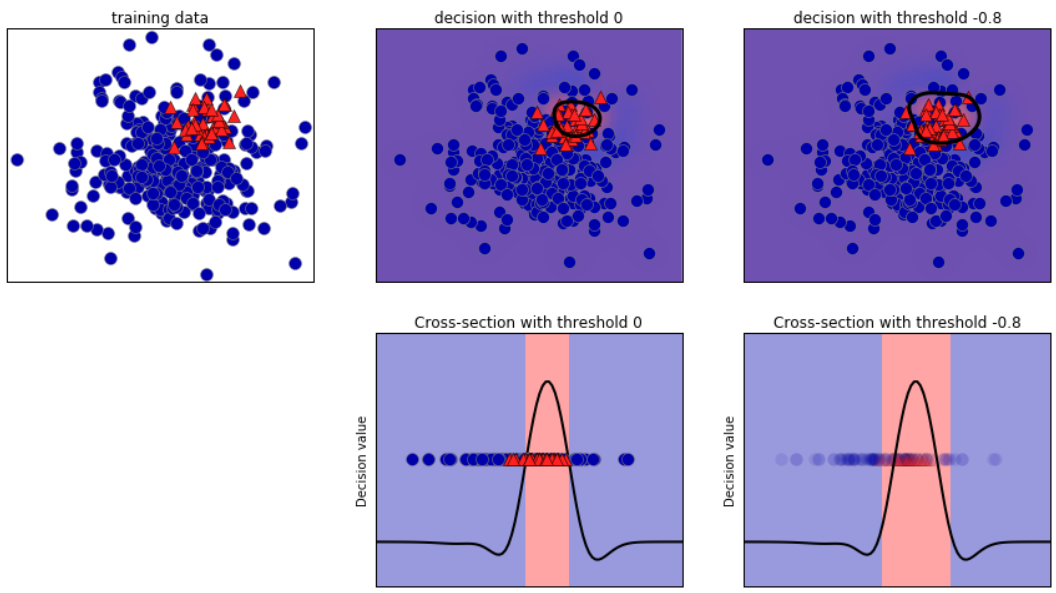
\includegraphics[scale=0.55]{Imagen_Machine/Impacto}
	\caption{Mapa caliente de la función de decisión y el impacto de la modificación del umbral de decisión}
	\label{Impacto}
\end{figure}



Podemos usar la función {\ttfamily classification\_report} para evaluar la precisión  y sensibilidad para ambas clases: 


\begin{lstlisting}%[frame=single]

In[51]:

   print(classification_report(y_test, svc.predict(X_test)))

Out[51]:

                 precision   recall   f1-score   support
                
             0        0.97     0.89       0.93       104
             1        0.35     0.67       0.46         9
       
   avg / total        0.92     0.88       0.89       113

\end{lstlisting}

Para la clase 1, obtenemos una sensibilidad  bastante pequeña, y la precisión es mixta. Debido
 a que la clase 0 es mucho más grande, el clasificador se centra en obtener la clase correcta, la 
  clase 0,  y no la clase 1 más pequeña. \\
  
Supongamos que en esta aplicación es más importante tener un valor alto de sensibilidad para la clase 1, como en el ejemplo de detección de cáncer anterior.     
  Esto significa que estamos dispuestos a arriesgar más falsos positivos (falsa clase 1) a cambio de más verdaderos positivos (lo que aumentará la sensibilidad). Las predicciones generadas por {\ttfamily svc.predict} realmente no cumplen con este requerimiento, pero podemos ajustar las predicciones para enfocarnos en una mayor sensibilidad de la clase 1, cambiando el umbral de decisión de 0. Por defecto, los puntos con un valor de {\ttfamily decision\_function}    superior a 0 se clasificarán como clase 1. 
  
  Queremos que se clasifiquen más puntos en la clase 1, por lo que necesitamos disminuir el umbral:


\begin{lstlisting}%[frame=single]

In[52]:

   y_pred_lower_threshold = svc.decision_function(X_test) > -.8

\end{lstlisting}

Veamos el reporte  de clasificación para esta predicción:


\begin{lstlisting}


In[53]:

   print(classification_report(y_test, y_pred_lower_threshold))

Out[53]:

               precision   recall   f1-score   support
               
            0       1.00     0.82       0.90       104
            1       0.32     1.00       0.49         9
            
  avg / total       0.95     0.83       0.87       113

\end{lstlisting}


Como se esperaba, la sensibilidad de la clase 1 aumentó y la precisión  disminuyó. 
Estamos ahora clasificando una región más grande del espacio como clase 1, como se ilustra en el gráfico superior derecho de Figura \ref{Impacto}.    Si evalúa  la precisión  sobre la sensibilidad o al revés, o sus datos son muy desbalanceados, cambiar el umbral de decisión es la forma más fácil de  obtener mejores  resultados.  Como {\ttfamily decision\_function}  puede  tener  rangos arbitrarios, es difícil proporcionar
una regla general sobre cómo elegir un umbral.\\


\begin{minipage}[t]{0.2\textwidth}
	\centering\raisebox{\dimexpr \topskip-\height}{%
		
\includegraphics[width=\textwidth]{Imagen_Machine/Escorpion}}
\end{minipage}%\hfill
\begin{minipage}[t]{0.75\textwidth} 
	{\scriptsize			
		Si configura un umbral, debe tener cuidado de no hacerlo usando el conjunto de prueba. Al igual que con cualquier otro parámetro, es probable que al configurar   un umbral de decisión en el conjunto de pruebas arroje resultados demasiado optimistas. En su lugar, use un conjunto de validación o validación cruzada.}
\end{minipage}\\



Elegir un umbral para  modelos que implementan el método {\ttfamily predic\_proba} puede ser
sencillo, ya que la salida de {\ttfamily predic\_proba} está en una escala fija de 0 a 1, y los modelos de probabilidad. Por defecto, el umbral de 0.5 significa que si el modelo es más del 50\%  "{}seguro"{}
que un punto es de la clase positiva, se clasificará como tal.   Aumentando el umbral significa que el modelo debe tener más confianza para tomar una decisión positiva (y menos confianza para tomar una decisión negativa).  

Trabajando con probabilidades puede ser más intuitivo que  trabajar con umbrales arbitrarios, no todos los modelos proporcionan modelos realistas de incertidumbre (un árbol de decisión que crece hasta lo más profundo es siempre 100\% seguro de sus decisiones, a pesar de que a menudo podría estar equivocado).  Esto  relaciona el concepto de calibración: un modelo calibrado es un modelo que proporciona una medidad de exactitud  de su incertidumbre.  Discutir la calibración en detalle está más allá del alcance  de  este  libro, pero puede encontrar más detalles en  el artículo \href{http://www.machinelearning.org/proceedings/icml2005/papers/079_GoodProbabilities_NiculescuMizilCaruana.pdf}{\color{vino} "{}Predicting Good Probabilities with   Supervised   Learning"{}} por   Alexandru  Niculescu-Mizil  and  Rich  Caruana.


\subsection{Precisión, sensibilidad  y curvas ROC}

% Precision-recall curves and ROC curves

Como acabamos de comentar, cambiar el umbral que se utiliza para hacer una clasificación decisión en un modelo es una forma de ajustar la compensación de precisión  y sensibilidad para una clasificación dada.
Tal vez quiera perder menos del 10\% de las muestras positivas, lo que significa que  desea una sensibilidad del  90\%.  Esta decisión depende de la aplicación, y debe ser impulsada por los objetivos del negocio.
Una vez que se configura un objetivo particular, por ejemplo, un    valor particular  de sensibilidad
  o de precisión para una clase: se puede establecer un umbral adecuadamente. Siempre es posible  configurar  un umbral  para cumplir un objetivo particular, como 90\% de sensibilidad.    Lo difícil es desarrollar un modelo  que  mantenga  una precisión  razonable con este umbral,  si  
clasifica todo como  positivo, tendrá un 100\% de sensibilidad, pero su modelo será inútil.\\

  Configurar  un requisito en un clasificador como 90\%  de  sensibilidad   con frecuencia  es llamado {\emph{ punto de operación}}.   La fijación de un {\emph{ punto de operación}}  es a menudo útil en  la configuración empresarial para dar garantías  de rendimiento a clientes u otros grupos dentro de su organización.\\

Generalmente, cuando se desarrollar un nuevo modelo, no está del todo claro cuál será el {\emph{ punto de operación}}. Por esta razón, y para entender mejor el problema de modelado, es instructivo observar  todos los umbrales posibles, o todas las posibles compensaciones entre precisión y sensibilidad a la vez. 
Esto es posible usando una herramienta llamada {\bf{curva de precisión-sensibilidad}}\index{curva de precisión-sensibilidad}. Se puede encontrar la función para calcular la curva exactitud-sensibilidad en el módulo {\ttfamily sklearn.metrics}. Necesita el etiquetado de la verdad fundamental y las incertidumbres predichas, creadas a través de {\ttfamily decision\_function} o {\ttfamily  predict\_proba}: 

\begin{lstlisting}%[frame=single]

In[54]:

   from sklearn.metrics import precision_recall_curve
   precision, recall, thresholds = precision_recall_curve(
       y_test, svc.decision_function(X_test))

\end{lstlisting}

La función {\ttfamily precision\_recall\_curve}  devuelve una lista de valores de precisión y sensibilidad para todos los umbrales posibles (todos los valores que aparecen en la función de decisión)  ordenados, para que podamos gráficar la curva, como se ve en la Figura \ref{Curva01}: 

\begin{lstlisting}%[frame=single]

In[55]:

   # Use more data points for a smoother curve
   X, y = make_blobs(n_samples=(4000, 500), centers=2, cluster_std=[7.0, 2],
                     random_state=22)
   X_train, X_test, y_train, y_test = train_test_split(X, y, random_state=0)
   svc = SVC(gamma=.05).fit(X_train, y_train)
   precision, recall, thresholds = precision_recall_curve(
       y_test, svc.decision_function(X_test))
   # find threshold closest to zero
   close_zero = np.argmin(np.abs(thresholds))
   plt.plot(precision[close_zero], recall[close_zero], 'o', markersize=10,
            label="threshold zero", fillstyle="none", c='k', mew=2)
            
   plt.plot(precision, recall, label="precision recall curve")
   plt.xlabel("Precision")
   plt.ylabel("Recall")

\end{lstlisting}


\begin{figure}[h!]
	\centering
	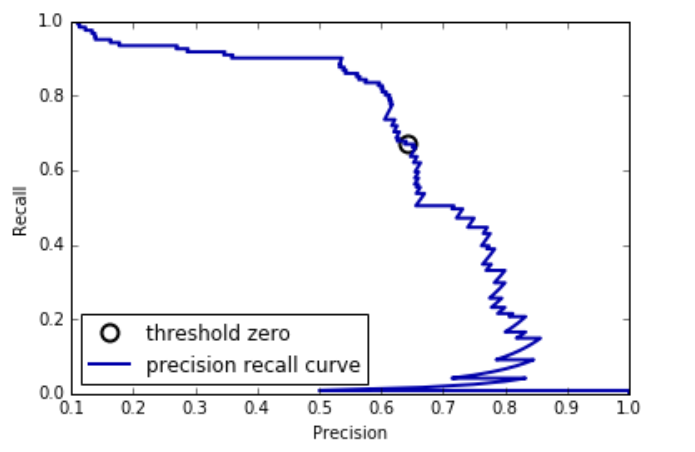
\includegraphics[scale=0.55]{Imagen_Machine/Curva01}
	\caption{Curva de precisión y sensibilidad   para SVC (gamma=0.05)}
	\label{Curva01}
\end{figure}

Cada punto a lo largo de la curva en la Figura \ref{Curva01}  corresponde a un posible umbral de la
{\ttfamily decisión\_función}. Podemos ver, por ejemplo, que se puede  lograr una  sensibilidad de 0.4 en una  precisión de aproximadamente 0,75.  El círculo negro marca el punto que corresponde a un umbral
 de 0, por defecto el umbral  para la {\ttfamily decisión\_función}. Este punto es la compensación que
se elige al llamar al método de predicción.


Cuanto más cerca se mantenga una curva de la esquina superior derecha, mejor será el clasificador. Un punto en la esquina superior derecha significa alta precisión y alta sensibilidad para el mismo umbral. 
La curva comienza en la esquina superior izquierda, corresponde  a un umbral muy bajo, clasificando
todo como la clase positiva.  Al elevar el umbral, la curva se mueve hacia una alta  precisión, pero también baja la sensibilidad. Subiendo el umbral cada vez más, llegamos a una  situación en la que la mayoría de los puntos  clasificados como positivos, son verdaderos positivos, lo que conduce a una muy alta precisión  pero menor sensibilidad.  Cuanto más el modelo mantiene  alta la sensibilidad  a medida que la precisión sube, lo mejor.


Si observamos   esta curva en particular un poco más, podemos ver que con este modelo es posible
 obtener una precisión   alrededor de 0,5 con una sensibilidad muy alta. Si queremos  mayor precisión, tenemos que sacrificar un poco de sensibilidad. En otras palabras,  la curva es relativamente
plana a la izquierda, lo que significa que la sensibilidad no baja mucho cuando necesitamos
mayor precisión. Para una precisión mayor a 0.5, cada ganancia en precisión nos cuesta un buena cantidad de  sensibilidad. \\
 
Los diferentes clasificadores pueden funcionar bien en diferentes partes de la curva, es decir, en diferentes puntos de operación.    Comparemos el modelo SVM  con el modelo de bosque aleatorio entrenados  en el mismo conjunto de datos.   El  {\ttfamily RandomForestClassifier} no tiene  {\ttfamily decision\_function}, sólo {\ttfamily  predic\_proba}.     La función {\ttfamily precision\_recall\_curve} espera como su segundo argumento   una medida de certeza para la clase positiva (clase 1), así que pasamos la probabilidad de que una muestra sea de clase 1, es decir, {\ttfamily rf.predict\_proba (X\_test)[:, 1]}.   El valor por defecto del umbral para {\ttfamily predic\_proba}  en la clasificación binaria es 0.5, entonces este es el punto marcado en la curva (ver Figura \ref{Curva02}):



\begin{lstlisting}%[frame=single]

In[56]:

   from sklearn.ensemble import RandomForestClassifier
   
   rf = RandomForestClassifier(n_estimators=100, random_state=0, 
                               max_features=2)
   rf.fit(X_train, y_train)
   
   # RandomForestClassifier has predict_proba, but not decision_function
   precision_rf, recall_rf, thresholds_rf = precision_recall_curve(
   y_test, rf.predict_proba(X_test)[:, 1])
   
   plt.plot(precision, recall, label="svc")
   
   plt.plot(precision[close_zero], recall[close_zero], 'o', markersize=10,
            label="threshold zero svc", fillstyle="none", c='k', mew=2)
   
   plt.plot(precision_rf, recall_rf, label="rf")
   
   close_default_rf = np.argmin(np.abs(thresholds_rf - 0.5))
   plt.plot(precision_rf[close_default_rf], recall_rf[close_default_rf], '^',
            c='k',  markersize=10, label="threshold 0.5 rf", 
            fillstyle="none", mew=2)            
   plt.xlabel("Precision")
   plt.ylabel("Recall")
   plt.legend(loc="best")

\end{lstlisting}



\begin{figure}[h!]
	\centering
	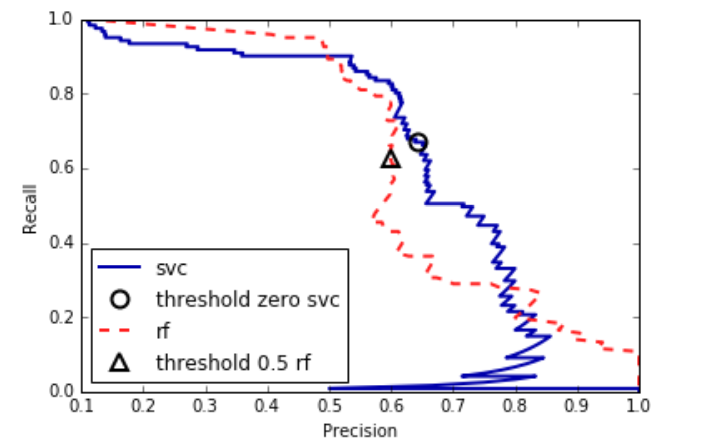
\includegraphics[scale=0.55]{Imagen_Machine/Curva02}
	\caption{Comparación de la  curvas de precisión-sensibilidad del SVM y bosque aleatorio}
	\label{Curva02}
\end{figure}


A partir de la gráfica de comparación podemos ver que el bosque aleatorio funciona mejor en los extremos, para una muy alta sensibilidad  o requisitos de precisión muy altos. Alrededor del  medio el SVM funciona mejor (aproximadamente una precisión = 0,7). Si sólo hubiéramos observado la $f_{1}$-puntuación  para comparar el rendimiento general, nos habríamos perdido estas sutilezas. La $f_{1}$-puntuación sólo captura un punto en la curva de precisión-sensibilidad, el que viene dado por el umbral por defecto:


\begin{lstlisting}%[frame=single]

In[57]:

   print("f1_score of random forest: {:.3f}".format(
          f1_score(y_test, rf.predict(X_test))))
   print("f1_score of svc: {:.3f}".format(
          f1_score(y_test, svc.predict(X_test))))

Out[57]:
   
    f1_score of random forest: 0.610
    f1_score of svc: 0.656

\end{lstlisting}



Comparando dos curvas de precisión-sensibilidad  proporciona gran cantidad de información detallada, pero es un proceso bastante manual. Para  comparar modelos automáticas, puede ser que queremos  resumir la información contenida en la curva, sin limitarnos a un umbral en particular   o  al  puntos de operación.
Una forma particular de resumir la curva precisión-sensibilidad,  es calculando la integral o el área bajo la curva de la curva de precisión-sensibilidad, también conocida como la \emph{precisión media}\footnote{\scriptsize	  Existen algunas diferencias técnicas menores entre el área bajo la curva de precisión-sensibilidad y la   precisión media. Sin embargo, esta explicación transmite la idea general.}. 
 Se puede usar la función {\ttfamily average\_precision\_score}  para calcular la precisión media.
Debido a que necesitamos calcular la curva ROC y considerar varios umbrales, el resultado de {\ttfamily decision\_function} o  {\ttfamily predict\_proba}  debe pasarse a {\ttfamily average\_precision\_score}, no el resultado de {\ttfamily predict}:



\begin{lstlisting}%[frame=single]

In[58]:
   
   from sklearn.metrics import average_precision_score
   ap_rf = average_precision_score(y_test, rf.predict_proba(X_test)[:, 1])
   ap_svc = average_precision_score(y_test, svc.decision_function(X_test))
   print("Average precision of random forest: {:.3f}".format(ap_rf))
   print("Average precision of svc: {:.3f}".format(ap_svc))

Out[58]:
   
    Average precision of random forest: 0.666
    Average precision of svc: 0.663

\end{lstlisting}


Al promediar todos los umbrales posibles, vemos que el bosque aleatorio y SVC
funcionan de manera similar, con el bosque aleatorio incluso un poco más adelante. Esto es muy diferente al  resultado que obtuvimos de {\ttfamily f1\_score} anteriormente.   Porque la precisión promedio es el área bajo una curva que va de 0 a 1, este siempre devuelve un valor  entre 0 (peor) y 1 (mejor). La precisión promedio de un clasificador que  asigna  {\ttfamily decision\_function}  al azar es la fracción de muestras positivas en el conjunto de datos.  


\subsubsection{Característica Operativa del Receptor (ROC) y el área bajo la curva  (AUC)}

% curva (ROC) de la característica operativa del receptor (n.f.)
%  recall (denominado igualmente sensibilidad o exhaustividad) 

Hay otra herramienta que se usa comúnmente para analizar el comportamiento de los clasificadores con
umbrales diferentes: la curva de característica operativa del receptor o la curva ROC. 

Similar a la curva de precisión-sensibilidad, la curva ROC considera todos los umbrales posibles para un clasificador dado, pero en lugar de reportar la precisión y sensibilidad, muestra la tasa de falsos positivos (false positive rate,  FPR) contra la tasa de verdaderos positivos (true positive rate, TPR). Recuerde  que la tasa verdaderos positivos  es simplemente otro nombre para la sensibilidad, mientras que la tasa falsos positivos es la fracción o tasa de falsos positivos de todas las muestras negativas:\\

$  FPR = \frac{FP }{FP+TN} $\\

%  Tasa de falsos positivos (FPR) se define de la siguiente manera:


La curva ROC puede calcularse utilizando la función {\ttfamily roc\_curve} (véase la figura \ref{Curva03}):

\begin{lstlisting}%[frame=single]

In[59]:

   from sklearn.metrics import roc_curve 
   fpr, tpr, thresholds = roc_curve(y_test, svc.decision_function(X_test))
   
   plt.plot(fpr, tpr, label="ROC Curve")
   plt.xlabel("FPR")
   plt.ylabel("TPR (recall)")
   # find threshold closest to zero
   close_zero = np.argmin(np.abs(thresholds))
   plt.plot(fpr[close_zero], tpr[close_zero], 'o', markersize=10,
            label="threshold zero", fillstyle="none", c='k', mew=2)
   plt.legend(loc=4)

\end{lstlisting}


\begin{figure}[h!]
	\centering
	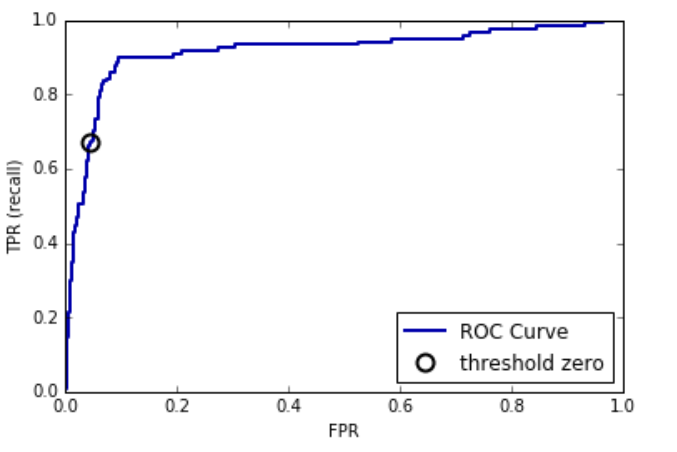
\includegraphics[scale=0.55]{Imagen_Machine/Curva03}
	\caption{Curva ROC para SVM}
	\label{Curva03}
\end{figure}


Para la característica operativa del receptor (ROC), la curva ideal está cerca de la parte superior izquierda: queremos  un  clasificador que produzca una alta sensibilidad  manteniendo una baja tasa de falsos positivos. 

En comparación con el umbral por defecto de 0, la curva muestra que podemos lograr una  sensibilidad significativamente mayor (alrededor de 0,9), mientras que sólo aumenta el FPR ligeramente.

El punto más cercano a la parte superior izquierda podría ser un mejor punto de operación que el elegido por defecto. Una vez más, tenga en cuenta que la elección de un umbral no debe hacerse en el conjunto de pruebas, sino en un conjunto de validación separado.
  
  %  puntos  operativo

En la Figura \ref{Curva04} se presenta  una comparación entre el bosque aleatorio y la SVM utilizando curvas ROC:

\begin{lstlisting}%[frame=single]

In[60]:

   from sklearn.metrics import roc_curve
   fpr_rf, tpr_rf, thresholds_rf = roc_curve(
            y_test, rf.predict_proba(X_test)[:, 1])
   
   plt.plot(fpr, tpr, label="ROC Curve SVC")
   plt.plot(fpr_rf, tpr_rf, label="ROC Curve RF")
   
   plt.xlabel("FPR")
   plt.ylabel("TPR (recall)")
   plt.plot(fpr[close_zero], tpr[close_zero], 'o', markersize=10,
            label="threshold zero SVC", fillstyle="none", c='k', mew=2)
   close_default_rf = np.argmin(np.abs(thresholds_rf - 0.5))
   plt.plot(fpr_rf[close_default_rf], tpr[close_default_rf], '^',
            markersize=10, label="threshold 0.5 RF", fillstyle="none",
            c='k', mew=2)
   
   plt.legend(loc=4)

\end{lstlisting}


\begin{figure}[h!]
	\centering
	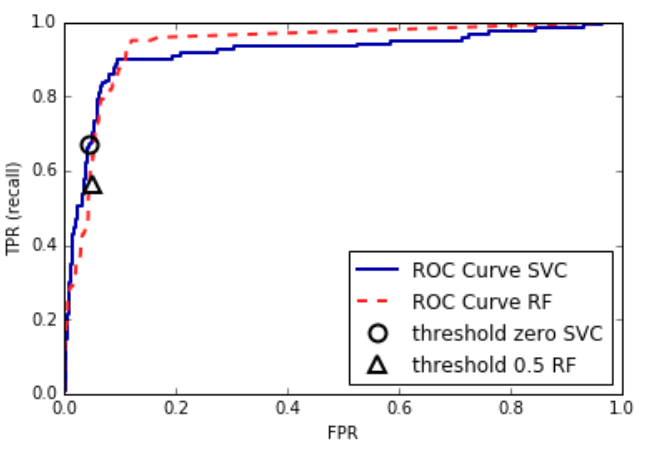
\includegraphics[scale=0.55]{Imagen_Machine/Curva04}
	\caption{Comparación de curvas ROC para SVM y bosque aleatorio}
	\label{Curva04}
\end{figure}


En cuanto a la curva precisión-sensibilidad, frecuentemente se quiere resumir la curva ROC usando 
un sólo número, el {\bf área bajo la curva} (esto se conoce comúnmente como AUC, y se entiende que la 
curva en cuestión es la curva ROC). Podemos comparar el área bajo la curva ROC usando la función
 {\ttfamily roc\_auc\_score}:

%Cuando se utilizan unidades normalizadas, el área bajo la curva (a menudo denominada simplemente AUC) es igual a la probabilidad de que un clasificador clasifique una instancia positiva elegida aleatoriamente por encima de una instancia negativa elegida aleatoriamente (asumiendo que 'positivo' clasifica por encima de ' negativo')

\begin{lstlisting}%[frame=single]

In[61]:

   from sklearn.metrics import roc_auc_score
   rf_auc = roc_auc_score(y_test, rf.predict_proba(X_test)[:, 1])
   svc_auc = roc_auc_score(y_test, svc.decision_function(X_test))
   print("AUC for Random Forest: {:.3f}".format(rf_auc))
   print("AUC for SVC: {:.3f}".format(svc_auc))

Out[61]:

    AUC for Random Forest: 0.937
    AUC for SVC: 0.916

\end{lstlisting}

%   Características de funcionamiento del receptor (ROC) y AUC 
%   Receiver operating characteristics (ROC) and AUC There 
%   Características operativas del receptor (ROC) y AUC

Comparando el bosque aleatorio y SVM usando el puntaje AUC, encontramos que el bosque aleatorio
funciona  mejor que el SVM. Recordemos eso porque la precisión media
 es el área bajo una curva que va de 0 a 1, la precisión media siempre retorna 
un valor entre 0 (peor) y 1 (mejor). La predicción aleatoria siempre produce un AUC
de 0.5, no importa qué tan desbalanceados  estén las clases en una dataset. 
Esto hace que AUC sea una  métrica mucho mejor para problemas de clasificación desbalanceada que la exactitud.  Las AUC puede interpretarse como una evaluación de la clasificación de muestras positivas. Es equivalente a la probabilidad de que un punto elegido al azar de la clase positiva tenga una puntuación más alta  según el clasificador que un punto elegido al azar de la clase negativa.   Así, un  AUC perfecto de 1 significa que todos los puntos positivos tienen una puntuación más alta que todos los negativos puntos.

Para problemas de clasificación con clases desbalanceadas, usando AUC para el modelo
 seleccinado suele ser mucho más significativa que usar la exactitud.

Volvamos al problema que estudiamos anteriormente de clasificar todos los nueves en dataset de dígitos
 versus todos los demás dígitos.  Clasificaremos la dataset con un SVM con tres diferentes
configuraciones  del ancho de banda del kernel, gamma (ver Figura \ref{Curva05}):


\begin{lstlisting}%[frame=single]

n[62]:

   y = digits.target == 9
   
   X_train, X_test, y_train, y_test = train_test_split(
       digits.data, y, random_state=0)
   
   plt.figure()
                    #  o   [1, 0.05, 0.01]:
   for gamma in [1, 0.1, 0.01]:         
       svc = SVC(gamma=gamma).fit(X_train, y_train)
       accuracy = svc.score(X_test, y_test)
       auc = roc_auc_score(y_test, svc.decision_function(X_test))
       fpr, tpr, _ = roc_curve(y_test , svc.decision_function(X_test))
       print("gamma = {:.2f} accuracy = {:.2f} AUC = {:.2f}".format(
             gamma, accuracy, auc))
   plt.plot(fpr, tpr, label="gamma={:.3f}".format(gamma))
   plt.xlabel("FPR")
   plt.ylabel("TPR")
   plt.xlim(-0.01, 1)
   plt.ylim(0, 1.02)
   plt.legend(loc="best")

Out[62]:

   gamma = 1.00 accuracy = 0.90 AUC = 0.50
   gamma = 0.1 accuracy = 0.90 AUC = 0.96
   gamma = 0.01 accuracy = 0.90 AUC = 1.00

\end{lstlisting}



\begin{figure}[h!]
	\centering
	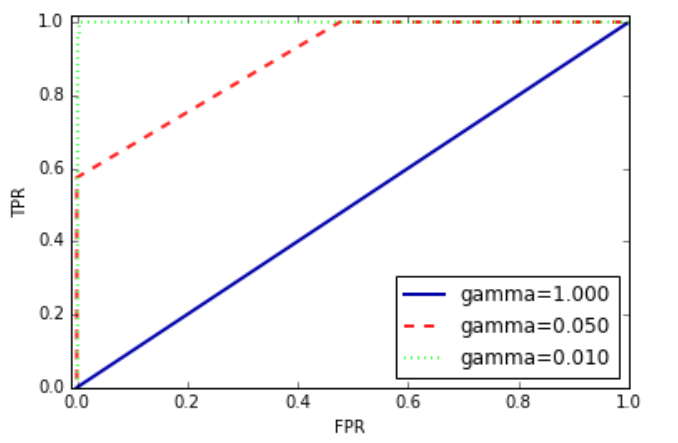
\includegraphics[scale=0.55]{Imagen_Machine/Curva05}
	\caption{curvas ROC para  SVMs con diferentes  configuraciones de gamma}
	\label{Curva05}
\end{figure}


La exactitud en las tres configuraciones de gamma es la misma, 90\%. Esto podría ser lo mismo
como un rendimiento casual, o tal vez no. Sin embargo,  observando las AUC y la curva  correspondiente,   
 vemos una clara distinción entre los tres modelos.  Con gamma = 1.0,
el AUC está realmente en el nivel de oportunidad o chance, lo que significa que la salida del {\ttfamily decision\_function} es tan buena como el aleatorio.  Con gamma = 0.01, el rendimiento mejora drásticamente de un AUC de 0.5 a 0.96. Finalmente, con gamma = 0.01, obtenemos un AUC perfecto igual a  1.0.   Eso significa que Todos los puntos positivos se clasifican más alto que todos los puntos negativos de acuerdo con la función de decisión. En otras palabras, con el umbral correcto, este modelo puede clasificar los datos perfectamente\footnote{\scriptsize  Observando la curva para {\ttfamily gamma=0.01} en detalle, se puede ver un pequeño giro cerca de la parte superior izquierda. Esto significa que al menos un punto no fue clasificado correctamente. La AUC de 1.0 es una consecuencia del redondeo al segundo punto decimal.}! 
Conociendo esto, podemos ajustar el umbral en este modelo y obtener excelentes predicciones.
Si solo hubiéramos usado la exactitud, nunca habríamos descubierto esto.  \\

Por esta razón, recomendamos usar AUC al evaluar modelos sobre dataset desbalanceadas.  Tenga en cuenta que AUC no utiliza el umbral predeterminado; sin embargo, puede ser necesario ajustar el umbral de decisión para obtener resultados de clasificación útiles a partir de un modelo con un AUC alto.

\subsection{Métricas para la clasificación multiclase}

Ahora que hemos discutido la evaluación de las tareas de clasificación binaria en profundidad, vamos a
pasar a las métricas para evaluar la clasificación multiclase. Básicamente, todas las métricas para
la clasificación multiclase se deriva de las métricas de clasificación binaria, pero promediado
sobre todas las clases.

La exactitud para la clasificación multiclase se define de nuevo como la fracción de ejemplos correctamente clasificados. Y de nuevo, cuando las clases están desbalanceadas, la exactitud no es una gran medida de evaluación. Imagine un problema de clasificación con tres clases con 85\% de puntos pertenecientes a la clase A, 10\% pertenecientes a la clase B y 5\% pertenecientes a la clase C.  ¿Qué significa ser 85\% exacto en este conjunto de datos? En general, los resultados de clasificación multiclase son más difíciles de entender que los resultados de clasificación binaria. Aparte de la exactitud, las dos herramientas más comunes son la matriz de confusión y el reporte de clasificación que vimos en el caso binario en la sección anterior. Vamos a aplicar estos dos métodos de evaluación detallada en la tarea de clasificar los 10  diferentes dígitos manuscritos en en la dataset de dígitos.



\begin{lstlisting}%[frame=single]

In[63]:

   from sklearn.metrics import accuracy_score
   X_train, X_test, y_train, y_test = train_test_split(
       digits.data, digits.target, random_state=0)
   lr = LogisticRegression().fit(X_train, y_train)
   pred = lr.predict(X_test)
   print("Accuracy: {:.3f}".format(accuracy_score(y_test, pred)))
   print("Confusion matrix:\n{}".format(confusion_matrix(y_test, pred)))

Out[63]:

    Accuracy: 0.953
    Confusion matrix:
    [[37 0 0 0 0 0 0 0 0 0]
     [ 0 39 0 0 0 0 2 0 2 0]
     [ 0 0 41 3 0 0 0 0 0 0]
     [ 0 0 1 43 0 0 0 0 0 1]
     [ 0 0 0 0 38 0 0 0 0 0]
     [ 0 1 0 0 0 47 0 0 0 0]
     [ 0 0 0 0 0 0 52 0 0 0]
     [ 0 1 0 1 1 0 0 45 0 0]
     [ 0 3 1 0 0 0 0 0 43 1]
     [ 0 0 0 1 0 1 0 0 1 44]]

\end{lstlisting}


El modelo tiene una exactitud del 95,3\%, lo que ya nos dice que lo estamos haciendo bastante bien. La matriz de confusión nos proporciona un poco más de detalle. En cuanto al caso binario, cada fila corresponde a una verdadera etiqueta, y cada columna corresponde a una etiqueta predicha. Puedes encontrar  visualización  más atractiva en la Figura \ref{ConfuM1}:


\begin{lstlisting}%[frame=single]

In[64]:

   scores_image = mglearn.tools.heatmap(
   confusion_matrix(y_test, pred), xlabel='Predicted label',
   ylabel='True label', xticklabels=digits.target_names,
   yticklabels=digits.target_names, cmap=plt.cm.gray_r, fmt="%d")
   plt.title("Confusion matrix")
   plt.gca().invert_yaxis()

\end{lstlisting}


\begin{figure}[h!]
	\centering
	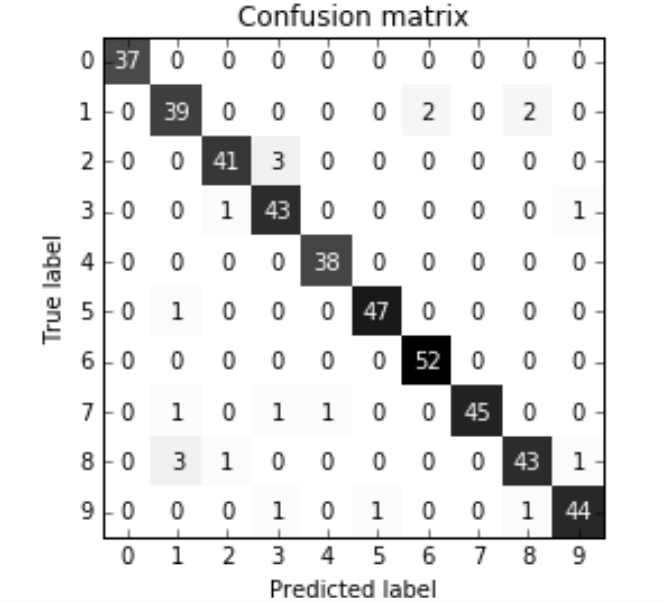
\includegraphics[scale=0.55]{Imagen_Machine/ConfuM1}
	\caption{Matriz de confusión para la tarea de clasificación de 10 dígitos}
	\label{ConfuM1}
\end{figure}

Para la primera clase, el dígito 0, hay 37 muestras en la clase, y todas estas muestras
 se clasificaron como clase 0 (no hay falsos negativos para la clase 0). Podemos ver eso
porque todas las demás entradas en la primera fila de la matriz de confusión son 0.
También podemos ver que ningún otro dígito se clasificó erróneamente como 0, porque todas las demás entradas en la primera columna de la matriz de confusión son 0 (no hay falsos positivos para la clase 0).
Sin embargo, algunos dígitos se confundieron con otros, por ejemplo, el dígito 2 (tercera fila),
tres de los cuales fueron clasificados como el dígito 3 (cuarta columna). También había un dígito
3 que se clasificó como 2 (cuarta fila, tercera columna) y un dígito 8 que se clasificó
como 2 (novena fila, tercera columna).

Con la función {\ttfamily classification\_report}, podemos calcular la precisión, sensibiidad,
y $f$-puntaje  para cada clase:


\begin{lstlisting}%[frame=single]

In[65]:

   print(classification_report(y_test, pred))

Out[65]:

               precision   recall   f1-score   support
    
             0      1.00     1.00       1.00        37
             1      0.89     0.91       0.90        43
             2      0.95     0.93       0.94        44
             3      0.90     0.96       0.92        45
             4      0.97     1.00       0.99        38
             5      0.98     0.98       0.98        48
             6      0.96     1.00       0.98        52
             7      1.00     0.94       0.97        48
             8      0.93     0.90       0.91        48
             9      0.96     0.94       0.95        47
             
   avg / total 0.95 0.95 0.95 450

\end{lstlisting}

Como era de esperar, la precisión y la sensibilidad son  perfectas, 1 para la clase 0, ya que no hay confusiones con esta clase. Por otro lado, para la clase 7,  la precisión es 1 porque no hay otra
la clase  clasificada  erróneamente como 7, mientras que para la clase 6 no hay falsos negativos, por lo que
el sensibilidad es 1. También podemos ver que el modelo tiene dificultades particulares con las clases 8
y la 3.

La métrica más utilizada para dataset desbalanceados  en la configuración de multiclase es
la versión multiclase del $f$-puntaje ($f$-score). La idea detrás del $f$-puntaje  multiclase es 
calcular un $f$-puntaje binario por clase, siendo esa clase la clase positiva y las otras
clases componen las clases negativa.

Luego, se promedian estos $f$-puntajes  por clase utilizando una de las siguientes estrategias:
 
 \begin{list}{$\bullet$}{}  
 \item el promedio "{}macro"{}  calcula  los  $f$-puntajes  no ponderados por clase. Esto da igual
 peso para todas las clases, sin importar su tamaño.

	\item  El promedio "{}ponderado"{}  calcula la media de los  $f$-puntajes  por clase, ponderada por
 su soporte. Esto es lo que se informa en el  reporte   de clasificación.
	
	\item   El promedio "{}micro"{}  calcula el número total de falsos positivos, falsos negativos,
 y verdaderos positivos sobre todas las clases, y luego calcula la precisión, la sensibilidad y el $f$-puntaje  utilizando estos recuentos.

\end{list}Si es importante cada muestra por igual, se recomienda utilizar el promedio "{}micro"{}  $f_{1}$-puntaje; o  si   cada clase es importante por igual, se recomienda usar el promedio "macro"
$f_{1}$-puntaje:

hsi te preocupas por cada clase por igual, se recomienda utilizar
la puntuación media "macro" f1:
\begin{lstlisting}%[frame=single]

In[66]:

   print("Micro average f1 score: {:.3f}".format(
          f1_score(y_test, pred, average="micro")))
   print("Macro average f1 score: {:.3f}".format(
          f1_score(y_test, pred, average="macro")))

Out[66]:

    Micro average f1 score: 0.953
    Macro average f1 score: 0.954

\end{lstlisting}




\subsection{Métricas para  regresión}

%  sobre-y sub-predicciones

La evaluación de la regresión se puede hacer con el mismo detalle que para la clasificación, por ejemplo,  analizando la predicción excesiva  o sobre-predicción (overpredicting) del objetivo versus la predicción insuficiente o sub-predicción (underpredicting).  Sin embargo, en la mayoría de las aplicaciones   que hemos visto, todos los regresores   usan  del  $R^{2}$  por defecto, y  el método de puntuación (score) es suficiente.

Algunas veces, las decisiones empresariales se toman en base al  error cuadrático medio o un error medio absoluto, lo que podría incentivar en afinar modelos utilizando estas métricas. Sin embargo, hemos encontrado que $R^{2}$ es una métrica más intuitiva para evaluar los modelos de regresión.





\section{Uso de métricas de evaluación en la selección del modelo}

% Using Evaluation Metrics in Model Selection


Hemos discutido muchos métodos de evaluación en detalle, y cómo aplicarlos dada la verdad fundamental y el modelo. Sin embargo, con frecuencia se quiere usar métricas como AUC en la selección de modelos mediante  {\ttfamily GridSearchCV} o {\ttfamily cross\_val\_score}. Por suerte {\ttfamily  scikit-learn} proporciona una manera muy simple de lograr esto, a través del argumento de puntuación que se puede utilizar tanto en {\ttfamily GridSearchCV} como en {\ttfamily cross\_val\_score}.   Simplemente  proporcionando una cadena que describa la métrica de evaluación que desea utilizar. Por ejemplo,  digamos  que queremos evaluar el clasificador SVM en la tarea "{}nueve vs. rest"{} en la dataset de dígitos, usando la puntuación AUC.   Cambiar la puntuación por defecto  (accuracy) a AUC se puede hacer proporcionando "{}{\ttfamily roc\_auc}"{} como el parámetro {\ttfamily scoring}: 
 
 
 
\begin{lstlisting}%[frame=single]
 
In[67]:
 
   # default scoring for classification is accuracy
   print("Default scoring: {}".format(
          cross_val_score(SVC(), digits.data, digits.target == 9)))
   # providing scoring="accuracy" doesn't change the results
   explicit_accuracy = cross_val_score(SVC(), digits.data, 
                                       digits.target == 9,
                                       scoring="accuracy")
   print("Explicit accuracy scoring: {}".format(explicit_accuracy))
   roc_auc = cross_val_score(SVC(), digits.data, digits.target == 9,
                             scoring="roc_auc")
   print("AUC scoring: {}".format(roc_auc))

Out[67]:
 
    Default scoring: [ 0.9 0.9 0.9]
    Explicit accuracy scoring: [ 0.9 0.9 0.9]
    AUC scoring: [ 0.994 0.99 0.996]
 
\end{lstlisting}
 
 
 Del mismo modo, podemos cambiar la métrica utilizada la selección del mejor parámetros en la {\ttfamily  Grid  SearchCV}:
 
 
 \begin{lstlisting}%[frame=single]
 
In[68]:

   X_train, X_test, y_train, y_test = train_test_split(
       digits.data, digits.target == 9, random_state=0)
   # we provide a somewhat bad grid to illustrate the point:
   param_grid = {'gamma': [0.0001, 0.01, 0.1, 1, 10]}
   # using the default scoring of accuracy:
   grid = GridSearchCV(SVC(), param_grid=param_grid)
   grid.fit(X_train, y_train)
   print("Grid-Search with accuracy")
   print("Best parameters:", grid.best_params_)
   print("Best cross-validation score (accuracy)): {:.3f}".format(
          grid.best_score_))
   print("Test set AUC: {:.3f}".format(
          roc_auc_score(y_test, grid.decision_function(X_test))))
   print("Test set accuracy: {:.3f}".format(grid.score(X_test, y_test)))
 
Out[68]:

   Grid-Search with accuracy
   Best parameters: {'gamma': 0.0001}
   Best cross-validation score (accuracy)): 0.970
   Test set AUC: 0.992
   Test set accuracy: 0.973
 
In[69]:

    # using AUC scoring instead:
    grid = GridSearchCV(SVC(), param_grid=param_grid, scoring="roc_auc")
    grid.fit(X_train, y_train)
    print("\nGrid-Search with AUC")
     print("Best parameters:", grid.best_params_)
    print("Best cross-validation score (AUC): {:.3f}".format(
           grid.best_score_))
    print("Test set AUC: {:.3f}".format(
           roc_auc_score(y_test, grid.decision_function(X_test))))
    print("Test set accuracy: {:.3f}".format(grid.score(X_test, y_test)))
 
 Out[69]:
 
    Grid-Search with AUC
    Best parameters: {'gamma': 0.01}
    Best cross-validation score (AUC): 0.997
    Test set AUC: 1.000
    Test set accuracy: 1.000
  
 \end{lstlisting}   Cuando se usa la exactitud (accuracy), se selecciona el parámetro {\ttfamily gamma = 0.0001}, mientras que {\ttfamily gamma = 0.01} es  seleccionado cuando se usa  AUC.  La  exactitud de la validación cruzada es coherente  con la exactitud  del conjunto de prueba  en ambos casos. Sin embargo, el uso de AUC encontró una mejor configuración de parámetros en  términos de AUC e incluso en términos de exactitud\footnote{\scriptsize	 Encontrar una solución de mayor exactitud usando AUC es probablemente una consecuencia de que la exactitud sea una mala medida del rendimiento del modelo en datos desbalanceados.}.\\
 
 
 Los valores más importantes para el parámetro de puntuación ({\ttfamily scoring}) para la clasificación son la exactitud (el valor por defecto); {\ttfamily roc\_auc} para el área bajo  la curva ROC; {\ttfamily average\_precision}  para el área bajo la curva de precision-sensibilidad; {\ttfamily  f1, f1\_macro, f1\_micro}  y  {\ttfamily  f1\_weighted } para el  $f_{1}$-puntuación binaria  y  las diferentes variantes ponderadas.   Para la regresión,  los valores  más comunes usados  son el valor $r^{2}$ para el puntaje $R^{2}$, {\ttfamily mean\_squared\_error} para el error cuadratico medio    y {\ttfamily mean\_squared\_error}  para error absoluto medio.  Puedes encontrar una lista completa de   argumentos admitidos en la   \href{https://scikit-learn.org/stable/modules/model_evaluation.html#the-scoring-parameter-defining-model-evaluation-rules}{\textcolor{vino}{documentación} } o revisando  el diccionario {\ttfamily SCORER}  definido en el módulo de {\ttfamily  metrics.scorer}:
 

 \begin{lstlisting}%[frame=single]
 
In[70]:

   from sklearn.metrics.scorer import SCORERS
   print("Available scorers:\n{}".format(sorted(SCORERS.keys())))
 
Out[70]:
 
   Available scorers:
   ['accuracy', 'adjusted_rand_score', 'average_precision', 'f1', 
    'f1_macro', 'f1_micro', 'f1_samples', 'f1_weighted', 'log_loss',
    'mean_absolute_error', 'mean_squared_error', 'median_absolute_error',
    'precision', 'precision_macro', 'precision_micro', 'precision_samples',
    'precision_weighted','r2', 'recall', 'recall_macro', 'recall_micro',
    'recall_samples', 'recall_weighted', 'roc_auc']

\end{lstlisting}
 
 
 
 
 
 
 \subsection{Resumen y perspectivas}
 
 En este capítulo discutimos la validación cruzada, la búsqueda de cuadrícula (grid search) y las métricas de evaluación, el  pilares en la evaluación y mejora de algoritmos de aprendizaje automático. Las herramientas  descrito en este capítulo, junto con los algoritmos descritos en los capítulos \ref{Cap2}  y \ref{Cap3},  son el pan y la mantequilla de cada profesional del aprendizaje automático.\\
 
 Hay dos puntos particulares que hicimos en este capítulo que justifican repetir,
 porque a menudo son ignorados por los nuevos profesionales. El primero tiene que ver con
 validación cruzada. La validación cruzada o el uso de un conjunto de pruebas  nos permiten evaluar un
 modelo de aprendizaje automático, ya que funcionará en el futuro.    Sin embargo, si usamos el conjunto de prueba  o validación cruzada para seleccionar un modelo o seleccionar parámetros del modelo, "{}usamos"{} la data de  prueba y usar los mismos datos para evaluar qué tan bien funcionará el modelo en el futuro  conducirá a estimaciones demasiado optimistas.   Por lo tanto, debemos recurrir a una división en la data de entrenamiento para la construcción de modelos, en datos de validación para la selección de modelos y parámetros,  y datos de prueba para la evaluación del modelo.  En lugar de una simple división, podemos reemplazar cada uno de estas divisiones con validación cruzada.  La forma más utilizada (como se describió anteriormente) es una división de entrenamiento{\scriptsize/}prueba para evaluación, y utiliza validación cruzada en el entrenamiento  configurado para el modelo y para la selección de los  parámetro.\\

 El segundo punto tiene que ver con la importancia de la métrica de evaluación o función de puntuación utilizada para la selección y evaluación de modelos. La teoría de cómo tomar decisiones comerciales a partir de las predicciones de un modelo de aprendizaje automático estan  más allá del alcance de este libro\footnote{\scriptsize Se recomienda  el libro de Foster Provost y Tom Fawcett \href{https://www.oreilly.com/library/view/data-science-for/9781449374273/}{\textcolor{vino}{Data Science for Business}}  (O'Reilly) para obtener más información sobre este tema.}.   Sin embargo, rara vez es el caso que el objetivo final de una tarea de aprendizaje automático sea construir un modelo con una alta exactitud.  Asegúrese de que  la métrica que elija para evaluar y seleccionar un modelo es un buen sustituto para lo  que el   modelo realmente se utilizará. En realidad, los problemas de clasificación rara vez tiene  clases balanceadas, y con frecuencia  falsos positivos y falsos negativos tienen consecuencias muy diferentes. En realidad, los problemas de clasificación rara vez tienen clases equilibradas, y a menudo falsos positivos y falsos negativos tienen consecuencias muy diferentes.  Asegúrese de comprender cuáles son estas consecuencias y elija una métrica de evaluación acorde.\\ 
 
 Las técnicas de evaluación y selección de modelos que hemos descrito hasta ahora son las herramientas más importantes en la caja de herramientas de un científico de datos.\\

 La búsqueda en cuadrícula (Grid search) y la validación cruzada como las hemos descrito en este capítulo sólo se pueden aplicar en un modelo supervisado.  Sin embargo, hemos visto antes que muchos modelos requieren preprocesamiento, y que en algunas aplicaciones, como el ejemplo de reconocimiento facial en el capítulo \ref{Cap3},   extraer una representación diferente de los datos puede ser útil. En el próximo capítulo, vamos a introducir la clase {\ttfamily Pipeline}, que nos permite utilizar la búsqueda en cuadrícula (grid search) y la validación cruzada en estas complejas cadenas de algoritmos.
 
 
 
 
 
 